\documentclass[11pt, a4paper]{article}

% --- Packages ---
\usepackage[margin=2.2cm, top=2.2cm, bottom=2.2cm]{geometry}
\usepackage{amsmath, amssymb}
\usepackage{booktabs, array}
\usepackage{enumitem}
\usepackage{xcolor}
\usepackage{titlesec}
\usepackage{tikz}
\usetikzlibrary{calc,3d}
\newcommand{\cosec}{\operatorname{cosec}}
\usepackage{parskip}

% --- Colors & Styling ---
% Mostly monochrome: near-black ink for structure, muted gray for secondary text,
% a single desaturated terracotta accent reserved for chapter titles, section
% rules, and key term highlights.
\definecolor{primary}{RGB}{30, 30, 30}
\definecolor{secondary}{RGB}{95, 95, 95}
\definecolor{accent}{RGB}{184, 108, 58}

% Section headers: small caps, ink-colored, thin accent rule beneath
\titleformat{\section}
  {\normalfont\Large\bfseries\scshape\color{primary}}
  {}{0em}
  {}
  [{\color{accent}\titlerule[0.8pt]}]
\titlespacing*{\section}{0pt}{1.4em}{0.6em}

% Subsection headers: italic muted gray, no rule (keeps hierarchy restrained)
\titleformat{\subsection}
  {\normalfont\large\bfseries\itshape\color{secondary}}
  {}{0em}
  {}
\titlespacing*{\subsection}{0pt}{1em}{0.4em}

% --- Document ---
\begin{document}

\begin{center}
    {\LARGE \bfseries \color{accent} Preface}\\
    \vspace{0.2cm}
    {\color{accent}\rule{0.55\linewidth}{0.8pt}}
\end{center}
\vspace{0.35cm}

This document is a condensed formulario derived from Joseph Edwards's \textit{A Treatise on the Integral Calculus with Applications, Examples and Problems}, Volume I (Macmillan and Co., 1921) --- a comprehensive classical reference on integral calculus, now in the public domain.

The intention here is modest: to compress the standard forms, reduction formulae, and key theorems scattered across Edwards's original text into a single, quick-reference formulario suitable for review --- in the spirit of preparation for integral bees, olympiads, or general brush-up. This is a modernization of presentation and notation, not a replacement. The original contains full derivations, worked examples, historical context, and extensive exercise sets that this summary intentionally omits; readers wanting rigor, proof, or practice problems should consult the source directly.

This formulario was condensed chapter by chapter with the help of AI summarization, then reviewed and restyled for readability. This is a theory-only reference: exercise lists have been removed entirely, since they could not be reliably transcribed through the summarization pipeline and are not presented here rather than risk showing incorrect problems. Given the volume of theoretical material involved, occasional transcription errors may still remain despite review; if a result looks suspicious, it is worth checking against the original.

Chapters II through XXII follow Edwards's original numbering so that cross-referencing the source text remains straightforward. Edwards's own Chapter I, \textit{Nature of the Problem --- Preliminary Considerations}, is not included here, as it covers historical and foundational material (fluents and fluxions, Newton's lemmas, early numerical methods such as Simpson's and Weddle's rules) rather than the standard forms and integration techniques this formulario focuses on. In its place, Chapter I of this document is a custom-built reference chapter, not from Edwards, collecting the trigonometric, hyperbolic, and logarithmic identities used throughout the rest of the formulario.

\newpage

\begin{center}
    {\LARGE \bfseries \color{accent} Chapter I: Trigonometric, Hyperbolic \& Logarithmic Identities}\\
    \vspace{0.2cm}
    {\color{accent}\rule{0.55\linewidth}{0.8pt}}
\end{center}
\vspace{0.35cm}

\section*{I. Fundamental Trigonometric Identities}

\begin{center}
\begin{tabular}{@{}p{0.3\linewidth} p{0.3\linewidth} p{0.3\linewidth}@{}}
\toprule
\textbf{Reciprocal} & \textbf{Quotient} & \textbf{Negative Angle} \\
\midrule
$\sin\alpha = \dfrac{1}{\csc\alpha}$ & $\tan\alpha = \dfrac{\sin\alpha}{\cos\alpha}$ & $\sin(-x) = -\sin x$ \\[2mm]
$\cos\alpha = \dfrac{1}{\sec\alpha}$ & $\cot\alpha = \dfrac{\cos\alpha}{\sin\alpha}$ & $\cos(-x) = \cos x$ \\[2mm]
$\tan\alpha = \dfrac{1}{\cot\alpha}$ & & $\tan(-x) = -\tan x$ \\
\bottomrule
\end{tabular}
\end{center}

\begin{center}
\begin{tabular}{@{}p{0.9\linewidth}@{}}
\toprule
\textbf{Pythagorean Identities} \\
\midrule
$\sin^2\alpha + \cos^2\alpha = 1, \qquad \sec^2\alpha = 1 + \tan^2\alpha, \qquad \csc^2\alpha = 1 + \cot^2\alpha$ \\
\bottomrule
\end{tabular}
\end{center}

\section*{II. Sum, Difference \& Multiple-Angle Formulas}

\begin{center}
\begin{tabular}{@{}p{0.47\linewidth} p{0.47\linewidth}@{}}
\toprule
\textbf{Sum} & \textbf{Difference} \\
\midrule
$\sin(\alpha+\beta)=\sin\alpha\cos\beta+\cos\alpha\sin\beta$ & $\sin(\alpha-\beta)=\sin\alpha\cos\beta-\cos\alpha\sin\beta$ \\[2mm]
$\cos(\alpha+\beta)=\cos\alpha\cos\beta-\sin\alpha\sin\beta$ & $\cos(\alpha-\beta)=\cos\alpha\cos\beta+\sin\alpha\sin\beta$ \\[2mm]
$\tan(\alpha+\beta)=\dfrac{\tan\alpha+\tan\beta}{1-\tan\alpha\tan\beta}$ & $\tan(\alpha-\beta)=\dfrac{\tan\alpha-\tan\beta}{1+\tan\alpha\tan\beta}$ \\[3mm]
$\cot(\alpha+\beta)=\dfrac{\cot\alpha\cot\beta-1}{\cot\beta+\cot\alpha}$ & $\cot(\alpha-\beta)=\dfrac{\cot\alpha\cot\beta+1}{\cot\beta-\cot\alpha}$ \\
\bottomrule
\end{tabular}
\end{center}

\begin{center}
\begin{tabular}{@{}p{0.4\linewidth} p{0.5\linewidth}@{}}
\toprule
\textbf{Double Angle} & \textbf{Half Angle} \\
\midrule
$\sin 2\alpha = 2\sin\alpha\cos\alpha$
& $\sin\dfrac{\alpha}{2} = \pm\sqrt{\dfrac{1-\cos\alpha}{2}}$ \\[3mm]

$\cos 2\alpha = \cos^2\alpha - \sin^2\alpha$
& $\cos\dfrac{\alpha}{2} = \pm\sqrt{\dfrac{1+\cos\alpha}{2}}$ \\[3mm]

$\tan 2\alpha = \dfrac{2\tan\alpha}{1-\tan^2\alpha}$
& $\tan\dfrac{\alpha}{2} = \pm\sqrt{\dfrac{1-\cos\alpha}{1+\cos\alpha}}$ \\[3mm]

$\cot 2\alpha = \dfrac{\cot^2\alpha-1}{2\cot\alpha}$
& $\cot\dfrac{\alpha}{2} = \pm\sqrt{\dfrac{1+\cos\alpha}{1-\cos\alpha}}$ \\[3mm]

$\sec 2\alpha = \dfrac{1+\tan^2\alpha}{1-\tan^2\alpha}$
& $\sec\dfrac{\alpha}{2} = \pm\sqrt{\dfrac{2}{1+\cos\alpha}}$ \\[3mm]

$\csc 2\alpha = \dfrac{1}{2}\left(\cot\alpha+\tan\alpha\right)$
& $\csc\dfrac{\alpha}{2} = \pm\sqrt{\dfrac{2}{1-\cos\alpha}}$ \\

\bottomrule
\end{tabular}
\end{center}

\begin{center}
\begin{tabular}{@{}p{0.9\linewidth}@{}}
\toprule
\textbf{Triple Angle} \\
\midrule
$\sin 3\alpha = 3\sin\alpha - 4\sin^3\alpha \qquad \cos 3\alpha = 4\cos^3\alpha - 3\cos\alpha \qquad \tan 3\alpha = \dfrac{3\tan\alpha - \tan^3\alpha}{1-3\tan^2\alpha}$ \\
\bottomrule
\end{tabular}
\end{center}

\section*{III. Cofunction, Reduction \& Power-Reduction Identities}

\begin{center}
\begin{tabular}{@{}p{0.3\linewidth} p{0.3\linewidth} p{0.3\linewidth}@{}}
\toprule
\multicolumn{3}{@{}l}{\textbf{Cofunction Identities}} \\
\midrule
$\sin\left(\frac{\pi}{2}-x\right)=\cos x$ & $\cos\left(\frac{\pi}{2}-x\right)=\sin x$ & $\tan\left(\frac{\pi}{2}-x\right)=\cot x$ \\[2mm]
$\csc\left(\frac{\pi}{2}-x\right)=\sec x$ & $\sec\left(\frac{\pi}{2}-x\right)=\csc x$ & $\cot\left(\frac{\pi}{2}-x\right)=\tan x$ \\
\bottomrule
\end{tabular}
\end{center}

\begin{center}
\begin{tabular}{@{}p{0.45\linewidth} p{0.45\linewidth}@{}}
\toprule
\textbf{Reduction ($\pi + x$)} & \textbf{Reduction ($\pi/2 + x$)} \\
\midrule
$\sin(x+\pi)=-\sin x$ & $\sin\left(\frac{\pi}{2}+x\right)=\cos x$ \\
$\cos(x+\pi)=-\cos x$ & $\cos\left(\frac{\pi}{2}+x\right)=-\sin x$ \\
$\tan(x+\pi)=\tan x$ & $\tan\left(\frac{\pi}{2}+x\right)=-\cot x$ \\
\bottomrule
\end{tabular}
\end{center}

\begin{center}
\begin{tabular}{@{}p{0.9\linewidth}@{}}
\toprule
\textbf{Power-Reduction Identities} \\
\midrule
$\sin^2\alpha = \dfrac{1-\cos 2\alpha}{2} \qquad \cos^2\alpha = \dfrac{1+\cos 2\alpha}{2} \qquad \tan^2\alpha = \dfrac{1-\cos 2\alpha}{1+\cos 2\alpha}$ \\
\bottomrule
\end{tabular}
\end{center}

\section*{IV. Sum-to-Product Formulas}

\begin{center}
\begin{tabular}{@{}p{0.45\linewidth} p{0.45\linewidth}@{}}
\toprule
\textbf{Sum} & \textbf{Difference} \\
\midrule
$\sin\alpha+\sin\beta = 2\sin\dfrac{\alpha+\beta}{2}\cos\dfrac{\alpha-\beta}{2}$ & $\sin\alpha-\sin\beta = 2\cos\dfrac{\alpha+\beta}{2}\sin\dfrac{\alpha-\beta}{2}$ \\[3mm]
$\cos\alpha+\cos\beta = 2\cos\dfrac{\alpha+\beta}{2}\cos\dfrac{\alpha-\beta}{2}$ & $\cos\alpha-\cos\beta = -2\sin\dfrac{\alpha+\beta}{2}\sin\dfrac{\alpha-\beta}{2}$ \\[3mm]
$\tan\alpha+\tan\beta = \dfrac{\sin(\alpha+\beta)}{\cos\alpha\cos\beta}$ & $\tan\alpha-\tan\beta = \dfrac{\sin(\alpha-\beta)}{\cos\alpha\cos\beta}$ \\
\bottomrule
\end{tabular}
\end{center}

\section*{V. Law of Sines, Cosines \& Tangent}

\begin{center}
\begin{tabular}{@{}p{0.3\linewidth} p{0.6\linewidth}@{}}
\toprule
\textbf{Law of Sines} & $\dfrac{a}{\sin A} = \dfrac{b}{\sin B} = \dfrac{c}{\sin C}$ \\
\midrule
\textbf{Law of Cosines} & $a^2 = b^2+c^2-2bc\cos A, \quad b^2 = a^2+c^2-2ac\cos B, \quad c^2 = a^2+b^2-2ab\cos C$ \\
\midrule
\textbf{Law of Tangents} & $\dfrac{a-b}{a+b} = \dfrac{\tan\frac{1}{2}(A-B)}{\tan\frac{1}{2}(A+B)}$ \\
\bottomrule
\end{tabular}
\end{center}

\section*{VI. Hyperbolic Function Identities}

\textit{Context: Hyperbolic functions mirror circular (trigonometric) functions closely, but with sign changes in several Pythagorean-type and double-angle identities. The table below lines up each pair.}

\begin{center}
\begin{tabular}{@{}p{0.45\linewidth} p{0.45\linewidth}@{}}
\toprule
\textbf{Hyperbolic} & \textbf{Trigonometric} \\
\midrule
$\sinh(-x) = -\sinh x$ & $\sin(-x) = -\sin x$ \\
$\cosh(-x) = \cosh x$ & $\cos(-x) = \cos x$ \\
$\tanh(-x) = -\tanh x$ & $\tan(-x) = -\tan x$ \\
\midrule
$\cosh^2 x - \sinh^2 x = 1$ & $\sin^2 x + \cos^2 x = 1$ \\
$\operatorname{sech}^2 x = 1 - \tanh^2 x$ & $\sec^2 x = 1 + \tan^2 x$ \\
$\operatorname{csch}^2 x = \coth^2 x - 1$ & $\csc^2 x = 1 + \cot^2 x$ \\
\midrule
$\sinh(x+y) = \sinh x\cosh y+\cosh x\sinh y$ & $\sin(x+y) = \sin x\cos y+\cos x\sin y$ \\
$\sinh(x-y) = \sinh x\cosh y-\cosh x\sinh y$ & $\sin(x-y) = \sin x\cos y-\cos x\sin y$ \\
$\sinh 2x = 2\sinh x\cosh x$ & $\sin 2x = 2\sin x\cos x$ \\
\midrule
$\cosh(x+y) = \cosh x\cosh y+\sinh x\sinh y$ & $\cos(x+y) = \cos x\cos y-\sin x\sin y$ \\
$\cosh(x-y) = \cosh x\cosh y-\sinh x\sinh y$ & $\cos(x-y) = \cos x\cos y+\sin x\sin y$ \\
$\cosh 2x = \cosh^2 x+\sinh^2 x$ & $\cos 2x = \cos^2 x-\sin^2 x$ \\
\midrule
$\tanh(x+y) = \dfrac{\tanh x+\tanh y}{1+\tanh x\tanh y}$ & $\tan(x+y) = \dfrac{\tan x+\tan y}{1-\tan x\tan y}$ \\[3mm]
$\tanh(x-y) = \dfrac{\tanh x-\tanh y}{1-\tanh x\tanh y}$ & $\tan(x-y) = \dfrac{\tan x-\tan y}{1+\tan x\tan y}$ \\[3mm]
\midrule
$\sinh^2 x = \dfrac{\cosh 2x - 1}{2}$ & $\sin^2 x = \dfrac{1-\cos 2x}{2}$ \\[2mm]
$\cosh^2 x = \dfrac{\cosh 2x + 1}{2}$ & $\cos^2 x = \dfrac{1+\cos 2x}{2}$ \\
\bottomrule
\end{tabular}
\end{center}

\section*{VII. Logarithmic Identities}

\begin{center}
\begin{tabular}{@{}p{0.45\linewidth} p{0.45\linewidth}@{}}
\toprule
\textbf{Definition} & \textbf{Exponent Form} \\
$\log_b x = a \iff x = b^a$ & $x^{\log_b a} = a^{\log_b x}$ \\
\midrule
\textbf{Same Base \& Argument} & \textbf{Argument One} \\
$\log_b b = 1 \quad (b>0,\, b\neq 1)$ & $\log_b 1 = 0 \quad (b>0,\, b\neq 1)$ \\
\midrule
\textbf{Product} & \textbf{Quotient} \\
$\log_b(xy) = \log_b x + \log_b y$ & $\log_b\!\left(\dfrac{x}{y}\right) = \log_b x - \log_b y$ \\[2mm]
\midrule
\textbf{Power of the Argument} & \textbf{Root of the Argument} \\
$\log_b(a^n) = n\log_b a$ & $\log_b \sqrt[n]{a} = \dfrac{1}{n}\log_b a$ \\[2mm]
\midrule
\textbf{Change of Base} & \textbf{Change of Base by Argument} \\
$\log_b a = \dfrac{\log_c a}{\log_c b}$ & $\log_b a = \dfrac{1}{\log_a b}$ \\[2mm]
\midrule
\textbf{Power of a Logarithm} & \textbf{Chain Rule} \\
$(\log_b a)^n \equiv \log_b^n a$ & $\log_b a \cdot \log_a c \cdot \log_c d = \log_b d$ \\
\bottomrule
\end{tabular}
\end{center}

\newpage

\begin{center}
    {\LARGE \bfseries \color{accent} Chapter II: Standard Forms \& Integration}\\
    \vspace{0.2cm}
    {\color{accent}\rule{0.55\linewidth}{0.8pt}}
\end{center}
\vspace{0.35cm}


\section*{\color{primary} I. Core Formulas \& Standard Forms}

\subsection*{\color{secondary} Algebraic, Exponential \& Logarithmic}
\begin{center}
\begin{tabular}{@{}p{0.45\columnwidth} p{0.45\columnwidth}@{}}
\toprule
\textbf{Power \& Linear} & \textbf{Exponential \& Log} \\
\midrule
$\int x^n dx = \frac{x^{n+1}}{n+1} \quad (n \neq -1)$ & $\int e^x dx = e^x$ \\
$\int x^{-1} dx = \log|x|$ & $\int a^x dx = \frac{a^x}{\log a}$ \\
$\int (ax+b)^n dx = \frac{(ax+b)^{n+1}}{a(n+1)}$ & $\int \frac{\phi'(x)}{\phi(x)} dx = \log|\phi(x)|$ \\
$\int \frac{dx}{ax+b} = \frac{1}{a} \log|ax+b|$ & $\int [\phi(x)]^n \phi'(x) dx = \frac{[\phi(x)]^{n+1}}{n+1}$ \\
\bottomrule
\end{tabular}
\end{center}

\vspace{0.3cm}

\subsection*{\color{secondary} Trigonometric \& Inverse Trigonometric}
\begin{center}
\begin{tabular}{@{}p{0.45\columnwidth} p{0.45\columnwidth}@{}}
\toprule
\textbf{Basic Trig} & \textbf{Inverse Trig \& Special} \\
\midrule
$\int \cos x dx = \sin x$ & $\int \frac{dx}{\sqrt{a^2-x^2}} = \sin^{-1}\frac{x}{a}$ \\
$\int \sin x dx = -\cos x$ & $\int \frac{dx}{a^2+x^2} = \frac{1}{a}\tan^{-1}\frac{x}{a}$ \\
$\int \sec^2 x dx = \tan x$ & $\int \frac{dx}{x\sqrt{x^2-a^2}} = \frac{1}{a}\sec^{-1}\frac{x}{a}$ \\
$\int \csc^2 x dx = -\cot x$ & $\int \frac{dx}{\sqrt{2ax-x^2}} = \cos^{-1}\frac{a-x}{a}$ \\
$\int \sec x \tan x dx = \sec x$ & $\int \tan x dx = \log|\sec x|$ \\
$\int \csc x \cot x dx = -\csc x$ & $\int \cot x dx = \log|\sin x|$ \\
\bottomrule
\end{tabular}
\end{center}

\vspace{0.3cm}

\subsection*{\color{secondary} General Laws of Integration}
\begin{itemize}[leftmargin=*, nosep]
    \item \textbf{\color{accent}Distributive:} $\int (u \pm v \pm w) dx = \int u dx \pm \int v dx \pm \int w dx$
    \item \textbf{\color{accent}Commutative (Constants):} $\int a u dx = a \int u dx$
    \item \textbf{\color{accent}Definite Integral:} $\int_a^b \phi(x) dx = y(b) - y(a)$
    \item \textbf{\color{accent}Inverse Notation:} $\int \phi(x) dx \equiv D^{-1}\phi(x)$
\end{itemize}


\section*{\color{primary} II. High-Yield Memory Rules}

\textbf{1. Dimensional Analysis Check}\\
If $x$ and $a$ are linear (dimension 1), $\frac{dx}{x}$ is dimensionless (0). Thus, $\int \frac{dx}{x} = \log x$ (dimensionless). Conversely, $\frac{dx}{a^2+x^2}$ has dimension $-1$. The result $\frac{1}{a}\tan^{-1}\frac{x}{a}$ correctly has dimension $-1$ because of the $\frac{1}{a}$ factor. Use this to instantly verify if a factor of $\frac{1}{a}$ is missing.

\textbf{2. The "co" Rule for Signs}\\
In trigonometry, if the integral's result begins with "co" ($\cos, \cot, \csc, \text{covers}$), it \textbf{must} have a negative sign. 
\textit{Examples:} $\int \sin x dx = -\cos x$, $\int \csc^2 x dx = -\cot x$. 
\textit{Note:} This does not apply to hyperbolic functions.

\newpage

\begin{center}
    {\LARGE \bfseries \color{accent} Chapter III: Change of the Independent Variable}\\
    \vspace{0.2cm}
    {\color{accent}\rule{0.55\linewidth}{0.8pt}}
\end{center}
\vspace{0.35cm}


\section*{\color{primary} I. Core Formulas \& Substitution Rules}

\subsection*{\color{secondary} General Substitution}
\begin{center}
\begin{tabular}{@{}p{0.45\columnwidth} p{0.45\columnwidth}@{}}
\toprule
\textbf{Indefinite Integral} & \textbf{Definite Integral} \\
\midrule
$\int f(x) dx = \int f(F(z)) F'(z) dz$ & $\int_a^b f(x) dx = \int_{F^{-1}(a)}^{F^{-1}(b)} f(F(z)) F'(z) dz$ \\
\bottomrule
\end{tabular}
\end{center}

\vspace{0.3cm}

\subsection*{\color{secondary} Standard Algebraic \& Trigonometric Substitutions}
\begin{center}
\begin{tabular}{@{}p{0.45\columnwidth} p{0.45\columnwidth}@{}}
\toprule
\textbf{Radical Form} & \textbf{Recommended Substitution} \\
\midrule
$\sqrt{a^2-x^2}$ & $x = a \sin \theta$ or $x = a \cos \theta$ \\
$\sqrt{a^2+x^2}$ & $x = a \tan \theta$ or $x = a \sinh z$ \\
$\sqrt{x^2-a^2}$ & $x = a \sec \theta$ or $x = a \cosh z$ \\
$\sqrt{2ax-x^2}$ & $x = a(1-\cos \theta)$ (Versine) \\
$\sqrt{a-x}$ or $\sqrt{a+x}$ & $x = a \cos 2\theta$ \\
$\sqrt{a^{2n} \pm x^{2n}}$ & $x^n = a^n \tan \theta$ or $x^n = a^n \sinh z$ \\
\bottomrule
\end{tabular}
\end{center}

\vspace{0.3cm}

\section*{\color{primary} II. Hyperbolic Functions \& Inverses}

\subsection*{\color{secondary} Definitions \& Complex Relations}
\begin{itemize}[leftmargin=*, nosep]
    \item $\sinh x = \frac{e^x - e^{-x}}{2}$, $\cosh x = \frac{e^x + e^{-x}}{2}$, $\tanh x = \frac{\sinh x}{\cosh x}$
    \item $\cosh^2 x - \sinh^2 x = 1$, $\cosh 2x = \cosh^2 x + \sinh^2 x$
    \item $\sin(ix) = i \sinh x$, $\cos(ix) = \cosh x$, $\tan(ix) = i \tanh x$
\end{itemize}

\subsection*{\color{secondary} Inverse Hyperbolic Functions (Logarithmic Forms)}
\begin{center}
\begin{tabular}{@{}p{0.45\columnwidth} p{0.45\columnwidth}@{}}
\toprule
\textbf{Inverse Function} & \textbf{Logarithmic Equivalent} \\
\midrule
$\sinh^{-1} \frac{x}{a}$ & $\log \left( \frac{x + \sqrt{x^2+a^2}}{a} \right)$ \\
$\cosh^{-1} \frac{x}{a}$ & $\log \left( \frac{x + \sqrt{x^2-a^2}}{a} \right)$ \\
$\tanh^{-1} \frac{x}{a}$ & $\frac{1}{2} \log \left( \frac{a+x}{a-x} \right) \quad (|x| < a)$ \\
$\coth^{-1} \frac{x}{a}$ & $\frac{1}{2} \log \left( \frac{x+a}{x-a} \right) \quad (|x| > a)$ \\
$\text{sech}^{-1} \frac{x}{a}$ & $\log \left( \frac{a + \sqrt{a^2-x^2}}{x} \right)$ \\
$\text{cosech}^{-1} \frac{x}{a}$ & $\log \left( \frac{a + \sqrt{a^2+x^2}}{x} \right)$ \\
\bottomrule
\end{tabular}
\end{center}

\vspace{0.3cm}

\subsection*{\color{secondary} The Gudermannian Function ($\text{gd}$)}
\textit{\small Context: A bridge between circular and hyperbolic functions without complex numbers. It naturally arises when integrating $\sec x$ and $\text{sech } x$.}
\vspace{0.15cm}

\begin{center}
\begin{tabular}{@{}p{0.45\columnwidth} p{0.45\columnwidth}@{}}
\toprule
\textbf{Definitions \& Inverses} & \textbf{The "Bridge" Identities} \\
\midrule
\textbf{\color{accent}Direct:} $\phi = \text{gd}(u)$ & $\sin(\text{gd } u) = \tanh u$ \\
$\phi = \int_0^u \text{sech } t \, dt = \arctan(\sinh u)$ & $\cos(\text{gd } u) = \text{sech } u$ \\
& $\tan(\text{gd } u) = \sinh u$ \\
\textbf{\color{accent}Inverse:} $u = \text{gd}^{-1}(\phi)$ & $\sinh(\text{gd}^{-1} \phi) = \tan \phi$ \\
$u = \int_0^\phi \sec \theta \, d\theta$ & $\cosh(\text{gd}^{-1} \phi) = \sec \phi$ \\
$u = \ln|\sec \phi + \tan \phi| = \ln \tan\left(\frac{\pi}{4}+\frac{\phi}{2}\right)$ & $\text{sech}(\text{gd}^{-1} \phi) = \cos \phi$ \\
\bottomrule
\end{tabular}
\end{center}

\vspace{0.2cm}

\begin{center}
\begin{tabular}{@{}p{0.45\columnwidth} p{0.45\columnwidth}@{}}
\toprule
\textbf{High-Yield Integrals (Bee/Olympiad)} & \textbf{Derivatives \& Properties} \\
\midrule
$\int \text{sech } x \, dx = \text{gd}(x) = \arctan(\sinh x)$ & $\frac{d}{du} \text{gd}(u) = \text{sech } u$ \\
$\int \sec x \, dx = \text{gd}^{-1}(x) = \ln|\sec x + \tan x|$ & $\frac{d}{d\phi} \text{gd}^{-1}(\phi) = \sec \phi$ \\
$\int \frac{dx}{\cosh x} = 2\arctan(e^x) - \frac{\pi}{2}$ & $\text{gd}(u) + \text{gd}(-u) = 0 \quad \text{(Odd function)}$ \\
$\int \frac{dx}{\cos x} = \ln\left|\tan\left(\frac{\pi}{4} + \frac{x}{2}\right)\right|$ & $\text{Range: } \text{gd}(u) \in \left(-\frac{\pi}{2}, \frac{\pi}{2}\right)$ \\
\bottomrule
\end{tabular}
\end{center}

\vspace{0.3cm}


\section*{\color{primary} III. Integrals of Quadratic Radicals}

\subsection*{\color{secondary} Integrals of $\frac{dx}{\sqrt{R}}$ where $R = ax^2+2bx+c$}
\begin{center}
\begin{tabular}{@{}p{0.45\columnwidth} p{0.45\columnwidth}@{}}
\toprule
\textbf{Condition} & \textbf{Result} \\
\midrule
$a > 0, b^2 < ac$ & $\frac{1}{\sqrt{a}} \sinh^{-1} \frac{ax+b}{\sqrt{ac-b^2}}$ \\
$a > 0, b^2 > ac$ & $\frac{1}{\sqrt{a}} \cosh^{-1} \frac{ax+b}{\sqrt{b^2-ac}}$ \\
$a < 0$ & $-\frac{1}{\sqrt{-a}} \sin^{-1} \frac{ax+b}{\sqrt{b^2-ac}}$ \\
\multicolumn{2}{c}{\textit{Universal Log Form (for $a>0$): } $\frac{1}{\sqrt{a}} \log(ax+b+\sqrt{aR})$} \\
\bottomrule
\end{tabular}
\end{center}

\vspace{0.3cm}

\section*{\color{primary} IV. Additional Standard Forms}

\begin{center}
\begin{tabular}{@{}p{0.45\columnwidth} p{0.45\columnwidth}@{}}
\toprule
\textbf{Hyperbolic \& Inverse} & \textbf{Algebraic \& Radical} \\
\midrule
$\int \cosh x dx = \sinh x$ & $\int \frac{dx}{\sqrt{x^2+a^2}} = \sinh^{-1}\frac{x}{a}$ \\
$\int \sinh x dx = \cosh x$ & $\int \frac{dx}{\sqrt{x^2-a^2}} = \cosh^{-1}\frac{x}{a}$ \\
$\int \text{sech}^2 x dx = \tanh x$ & $\int \sqrt{a^2-x^2} dx = \frac{x}{2}\sqrt{a^2-x^2} + \frac{a^2}{2}\sin^{-1}\frac{x}{a}$ \\
$\int \text{cosech}^2 x dx = -\coth x$ & $\int \sqrt{a^2+x^2} dx = \frac{x}{2}\sqrt{a^2+x^2} + \frac{a^2}{2}\sinh^{-1}\frac{x}{a}$ \\
$\int \text{sech} x \tanh x dx = -\text{sech} x$ & $\int \sqrt{x^2-a^2} dx = \frac{x}{2}\sqrt{x^2-a^2} - \frac{a^2}{2}\cosh^{-1}\frac{x}{a}$ \\
$\int \text{cosech} x \coth x dx = -\text{cosech} x$ & $\int \frac{dx}{x\sqrt{a^2-x^2}} = -\frac{1}{a}\text{sech}^{-1}\frac{x}{a}$ \\
$\int \frac{dx}{a^2-x^2} = \frac{1}{a}\tanh^{-1}\frac{x}{a} \ (x<a)$ & $\int \frac{dx}{x\sqrt{a^2+x^2}} = -\frac{1}{a}\text{cosech}^{-1}\frac{x}{a}$ \\
$\int \frac{dx}{x^2-a^2} = -\frac{1}{a}\coth^{-1}\frac{x}{a} \ (x>a)$ & $\int \frac{dx}{\sqrt{a^2-x^2}} = \sin^{-1}\frac{x}{a}$ \\
\bottomrule
\end{tabular}
\end{center}

\vspace{0.3cm}

\section*{\color{primary} V. High-Yield Memory Rules}

\textbf{1. The "co" Rule for Signs}\\
In trigonometry, if the integral's result begins with "co" ($\cos, \cot, \csc, \text{covers}$), it \textbf{must} have a negative sign. \textit{Note:} This does not apply to hyperbolic functions (e.g., $\int \sinh x dx = \cosh x$ is positive).

\textbf{2. Hyperbolic vs. Circular Analogy}\\
Hyperbolic integrals often mirror circular integrals but without the alternating signs. For example, $\int \frac{dx}{\sqrt{x^2-a^2}} = \cosh^{-1}\frac{x}{a}$ mirrors $\int \frac{dx}{\sqrt{a^2-x^2}} = \sin^{-1}\frac{x}{a}$. The Gudermannian $\theta = \text{gd } u$ perfectly maps circular functions of $\theta$ to hyperbolic functions of $u$.

\newpage

\begin{center}
    {\LARGE \bfseries \color{accent} Chapter IV: Integration by Parts \& Powers of Sines/Cosines}\\
    \vspace{0.2cm}
    {\color{accent}\rule{0.55\linewidth}{0.8pt}}
\end{center}
\vspace{0.35cm}


\section*{\color{primary} I. Integration by Parts}

\subsection*{\color{secondary} Core Formulas}
\begin{center}
\begin{tabular}{@{}p{0.45\columnwidth} p{0.45\columnwidth}@{}}
\toprule
\textbf{Standard Formula} & \textbf{General Rule (Repeated Parts)} \\
\midrule
$\int u \, dv = uv - \int v \, du$ & $\int u v \, dx = u v_1 - u' v_2 + u'' v_3 - \dots + (-1)^{n-1} u^{(n-1)} v_n + (-1)^n \int u^{(n)} v_n \, dx$ \\
\bottomrule
\end{tabular}
\end{center}

\vspace{0.2cm}

\textbf{\color{accent}\small Context:} Choose $u$ to be the function that simplifies when differentiated (e.g., polynomials, logs, inverse trig), and $dv$ to be the easily integrable part (e.g., exponentials, trig). Remember the mnemonic \textbf{LIATE} (Logarithmic, Inverse trig, Algebraic, Trig, Exponential).

\vspace{0.3cm}

\section*{\color{primary} II. Exponential-Trigonometric Integrals}

\begin{center}
\begin{tabular}{@{}p{0.45\columnwidth} p{0.45\columnwidth}@{}}
\toprule
\textbf{Sine Form} & \textbf{Cosine Form} \\
\midrule
$\int e^{ax} \sin bx \, dx = \frac{e^{ax}}{a^2+b^2} (a \sin bx - b \cos bx)$ & $\int e^{ax} \cos bx \, dx = \frac{e^{ax}}{a^2+b^2} (a \cos bx + b \sin bx)$ \\
\bottomrule
\end{tabular}
\end{center}

\vspace{0.2cm}

\textbf{\color{accent}\small Context:} Derived by applying parts twice and solving for the original integral, or by using complex exponentials ($\int e^{(a+ib)x} dx$). Highly frequent in Olympiad differential equations.

\vspace{0.3cm}

\section*{\color{primary} III. Reduction Formulae}

\subsection*{\color{secondary} Trigonometric Reductions}
\begin{center}
\begin{tabular}{@{}p{0.45\columnwidth} p{0.45\columnwidth}@{}}
\toprule
\textbf{Sine \& Cosine} & \textbf{Tangent \& Secant} \\
\midrule
$\int \sin^n x \, dx = -\frac{\sin^{n-1} x \cos x}{n} + \frac{n-1}{n} \int \sin^{n-2} x \, dx$ & $\int \tan^n x \, dx = \frac{\tan^{n-1} x}{n-1} - \int \tan^{n-2} x \, dx$ \\
$\int \cos^n x \, dx = \frac{\cos^{n-1} x \sin x}{n} + \frac{n-1}{n} \int \cos^{n-2} x \, dx$ & $\int \sec^n x \, dx = \frac{\sec^{n-2} x \tan x}{n-1} + \frac{n-2}{n-1} \int \sec^{n-2} x \, dx$ \\
\bottomrule
\end{tabular}
\end{center}

\vspace{0.2cm}

\textbf{\color{accent}\small Context:} A recursive technique that lowers the power/degree of an integrand step-by-step until it reaches a known base case. Essential for Olympiad problems with large exponents or limits like $\int_0^{\pi/2} \sin^n x \, dx$ (Wallis' Integrals).

\subsection*{\color{secondary} Algebraic \& Logarithmic Reductions}
\begin{center}
\begin{tabular}{@{}p{0.45\columnwidth} p{0.45\columnwidth}@{}}
\toprule
\textbf{Polynomial $\times$ Trig} & \textbf{Polynomial $\times$ Log} \\
\midrule
$\int x^m \sin nx \, dx = -\frac{x^m \cos nx}{n} + \frac{m}{n} \int x^{m-1} \cos nx \, dx$ & $\int x^m \log^n x \, dx = \frac{x^{m+1} \log^n x}{m+1} - \frac{n}{m+1} \int x^m \log^{n-1} x \, dx$ \\
\bottomrule
\end{tabular}
\end{center}

\vspace{0.3cm}

\section*{\color{primary} IV. Powers of Sines and Cosines}

\begin{center}
\begin{tabular}{@{}p{0.45\columnwidth} p{0.45\columnwidth}@{}}
\toprule
\textbf{Odd Powers} & \textbf{Even Powers} \\
\midrule
$\int \sin^{2k+1} x \, dx = \int (1-\cos^2 x)^k \sin x \, dx$ & $\sin^2 x = \frac{1-\cos 2x}{2}, \quad \cos^2 x = \frac{1+\cos 2x}{2}$ \\
Let $u = \cos x \implies du = -\sin x \, dx$ & $\sin x \cos x = \frac{\sin 2x}{2}, \quad \sin^2 x \cos^2 x = \frac{\sin^2 2x}{4}$ \\
\bottomrule
\end{tabular}
\end{center}

\vspace{0.2cm}

\textbf{\color{accent}\small Context:} For odd powers, peel off one factor and use $\sin^2+\cos^2=1$ for a $u$-substitution. For even powers, use half-angle identities to linearize the integrand into multiple angles (or use De Moivre's theorem).

\vspace{0.3cm}

\section*{\color{primary} V. Integration of Inverse Functions}

\begin{center}
\begin{tabular}{@{}p{0.9\columnwidth}@{}}
\toprule
\textbf{\color{accent}Formula:} $\int \phi^{-1}(x) \, dx = x \phi^{-1}(x) - \int \phi(y) \, dy \quad \text{(where } x = \phi(y)\text{)}$ \\
\bottomrule
\end{tabular}
\end{center}

\vspace{0.2cm}

\textbf{\color{accent}\small Context:} Geometrically, the area under an inverse function $y = f^{-1}(x)$ is the bounding rectangle minus the area to the left of the curve ($x = f(y)$).


\newpage

\begin{center}
    {\LARGE \bfseries \color{accent} Chapter V: Rational Algebraic Fractional Forms}\\
    \vspace{0.2cm}
    {\color{accent}\rule{0.55\linewidth}{0.8pt}}
\end{center}
\vspace{0.35cm}


\section*{\color{primary} I. Core Formulas for Rational Fractions}

\subsection*{\color{secondary} Difference of Squares}
\begin{center}
\begin{tabular}{@{}p{0.45\columnwidth} p{0.45\columnwidth}@{}}
\toprule
\textbf{Form} & \textbf{Integral} \\
\midrule
$\int \frac{dx}{a^2-x^2} \quad (|x|<a)$ & $\frac{1}{a} \tanh^{-1}\frac{x}{a} = \frac{1}{2a} \log \frac{a+x}{a-x}$ \\
$\int \frac{dx}{x^2-a^2} \quad (|x|>a)$ & $-\frac{1}{a} \coth^{-1}\frac{x}{a} = \frac{1}{2a} \log \frac{x-a}{x+a}$ \\
\bottomrule
\end{tabular}
\end{center}

\vspace{0.3cm}

\subsection*{\color{secondary} General Quadratic Denominator: $\int \frac{dx}{ax^2+bx+c}$}
\textit{\small Context: Complete the square to reduce to standard forms. The nature of the result depends on the discriminant $\Delta = b^2-4ac$.}
\vspace{0.15cm}
\begin{center}
\begin{tabular}{@{}p{0.45\columnwidth} p{0.45\columnwidth}@{}}
\toprule
\textbf{Case I: $b^2 < 4ac$} & \textbf{Case II: $b^2 > 4ac$} \\
\midrule
$\frac{2}{\sqrt{4ac-b^2}} \tan^{-1} \frac{2ax+b}{\sqrt{4ac-b^2}}$ & $\frac{1}{\sqrt{b^2-4ac}} \log \frac{2ax+b-\sqrt{b^2-4ac}}{2ax+b+\sqrt{b^2-4ac}}$ \\
\bottomrule
\end{tabular}
\end{center}

\vspace{0.3cm}

\subsection*{\color{secondary} Linear Numerator: $\int \frac{px+q}{ax^2+bx+c} dx$}
\textit{\small Context: Split the numerator into the derivative of the denominator and a constant.}
\begin{align*}
    px+q &= \frac{p}{2a}(2ax+b) + \left(q - \frac{pb}{2a}\right) \\
    \int \frac{px+q}{ax^2+bx+c} dx &= \frac{p}{2a} \log|ax^2+bx+c| + \left(q - \frac{pb}{2a}\right) \int \frac{dx}{ax^2+bx+c}
\end{align*}


\section*{\color{primary} II. Method of Partial Fractions}

\textit{\small Context: Decomposes a complex rational function $\frac{f(x)}{\phi(x)}$ into simpler fractions. The integral of any rational function is always expressible in finite terms (algebraic, logarithmic, and inverse trigonometric).}

\subsection*{\color{secondary} Decomposition Rules}
\begin{center}
\begin{tabular}{@{}p{0.45\columnwidth} p{0.45\columnwidth}@{}}
\toprule
\textbf{Factor in Denominator} & \textbf{Partial Fraction Form} \\
\midrule
Linear $(x-a)$ & $\frac{A}{x-a}$, where $A = \left. \frac{f(x)}{\phi(x)/(x-a)} \right|_{x=a}$ \\
Repeated Linear $(x-a)^r$ & $\frac{A_1}{x-a} + \frac{A_2}{(x-a)^2} + \dots + \frac{A_r}{(x-a)^r}$ \\
Irreducible Quadratic $(x^2+px+q)$ & $\frac{Px+Q}{x^2+px+q}$ \\
\bottomrule
\end{tabular}
\end{center}

\vspace{0.2cm}

\textit{\small Context for Repeated Factors: To find coefficients for $(x-a)^r$, substitute $x = a+y$ and expand $\frac{f(a+y)}{\phi(a+y)}$ in ascending powers of $y$ using long division or Taylor's theorem.}

\vspace{0.2cm}

\textit{\small Context for Irreducible Quadratics: When the denominator has real quadratic factors that cannot be factored into real linear terms ($\Delta < 0$), the partial fraction $\frac{Px+Q}{x^2+px+q}$ yields a mix of logarithmic and arctangent terms in the final integral.}

\section*{\color{primary} III. Special Rational \& Radical Forms}

\subsection*{\color{secondary} Binomial Denominators}
\begin{center}
\begin{tabular}{@{}p{0.9\columnwidth}@{}}
\toprule
$\int \frac{x^{m} dx}{x^{2n} - 2a^n x^n \cos \alpha + a^{2n}}$ \\
\bottomrule
\end{tabular}
\end{center}
\vspace{0.15cm}
\textit{\small Context: Solved by factoring the denominator using the $2n$-th roots of unity. The result is a finite sum of logarithms and arctangents.}

\subsection*{\color{secondary} Rationalizing Substitutions}
\begin{center}
\begin{tabular}{@{}p{0.45\columnwidth} p{0.45\columnwidth}@{}}
\toprule
\textbf{Integrand Form} & \textbf{Substitution} \\
\midrule
$\int \frac{x^{p-1} dx}{c+dx^q}$ & $x^q = z^l$ (where $l$ is LCM of denominators of fractional powers) \\
$\int f\left(\frac{a+bx}{c+dx}\right) dx$ & $\frac{a+bx}{c+dx} = z^l$ \\
\bottomrule
\end{tabular}
\end{center}

\newpage

\begin{center}
    {\LARGE \bfseries \color{accent} Chapter VI: Integral Forms involving Trigonometric Polynomials}\\
    \vspace{0.2cm}
    {\color{accent}\rule{0.55\linewidth}{0.8pt}}
\end{center}
\vspace{0.35cm}


\section*{\color{primary} I. Core Formulas for $\int \frac{dx}{a+b\cos x+c\sin x}$}

\textit{\small Context: The linear combination $b\cos x + c\sin x$ can be written as $R\cos(x-\gamma)$, where $R=\sqrt{b^2+c^2}$ and $\tan\gamma = c/b$. This reduces the integral to the standard form $\int \frac{dx}{a+R\cos(x-\gamma)}$.}

\subsection*{\color{secondary} Standard Results for $\int \frac{dx}{a+R\cos \theta}$}
\begin{center}
\begin{tabular}{@{}p{0.45\columnwidth} p{0.45\columnwidth}@{}}
\toprule
\textbf{Case I: $a^2 > R^2$} & \textbf{Case II: $a^2 < R^2$} \\
\midrule
$\frac{2}{\sqrt{a^2-R^2}} \tan^{-1} \left( \sqrt{\frac{a-R}{a+R}} \tan \frac{\theta}{2} \right)$ & $\frac{1}{\sqrt{R^2-a^2}} \log \frac{\sqrt{R+a} + \sqrt{R-a}\tan\frac{\theta}{2}}{\sqrt{R+a} - \sqrt{R-a}\tan\frac{\theta}{2}}$ \\
\bottomrule
\end{tabular}
\end{center}

\vspace{0.2cm}

\textit{\small Note: For $\int \frac{dx}{a+b\cos x+c\sin x}$, substitute $\theta = x-\gamma$ into the above forms. If $a^2 = R^2$, the integral evaluates to $-\frac{2}{a} \cot \frac{\theta}{2}$.}

\section*{\color{primary} II. Symmetrical Forms (Greenhill's Method)}

\textit{\small Context: Expresses the integral purely in terms of the integrand $y$. Highly elegant for evaluating definite integrals or when the integrand itself appears in the bounds, avoiding half-angle substitutions.}

\begin{center}
\begin{tabular}{@{}p{0.45\columnwidth} p{0.45\columnwidth}@{}}
\toprule
\textbf{Cosine Form ($b > a$)} & \textbf{Cosine Form ($b < a$)} \\
\midrule
$\int \frac{dx}{a+b\cos x} = \frac{1}{\sqrt{b^2-a^2}} \cosh^{-1} \frac{b+a\cos x}{a+b\cos x}$ & $\int \frac{dx}{a+b\cos x} = \frac{1}{\sqrt{a^2-b^2}} \cos^{-1} \frac{b+a\cos x}{a+b\cos x}$ \\
\midrule
\textbf{Sine Form ($b > a$)} & \textbf{Sine Form ($b < a$)} \\
\midrule
$\int \frac{dx}{a+b\sin x} = \frac{1}{\sqrt{b^2-a^2}} \cosh^{-1} \frac{b+a\sin x}{a+b\sin x}$ & $\int \frac{dx}{a+b\sin x} = \frac{1}{\sqrt{a^2-b^2}} \sin^{-1} \frac{b+a\sin x}{a+b\sin x}$ \\
\bottomrule
\end{tabular}
\end{center}


\section*{\color{primary} III. Reduction Formulae}

\textit{\small Context: Recursively lowers the power $n$ of the denominator. Crucial for Olympiad problems with large exponents or when evaluating integrals over symmetric intervals.}

\subsection*{\color{secondary} For $I_n = \int \frac{dx}{(a+b\cos x)^n}$}
\begin{align*}
    (n-1)(a^2-b^2) I_n &= \frac{b \sin x}{(a+b\cos x)^{n-1}} + (2n-3)a I_{n-1} - (n-2) I_{n-2}
\end{align*}

\subsection*{\color{secondary} For $I_n = \int \frac{dx}{(a+b\cos x+c\sin x)^n}$}
\begin{align*}
    (n-1)(a^2-b^2-c^2) I_n &= \frac{-b\sin x+c\cos x}{(a+b\cos x+c\sin x)^{n-1}} \\
    &\quad + (2n-3)a I_{n-1} - (n-2) I_{n-2}
\end{align*}

\subsection*{\color{secondary} For $I_{m,n} = \int \frac{\sin^m x}{(a+b\cos x)^n} dx$}
\textit{\small Context: Connects integrals with varying powers of sine in the numerator and the denominator.}
\begin{align*}
    b I_{m,n} &= -\frac{\sin^{m+1} x}{(n-1)(a^2-b^2)(a+b\cos x)^{n-1}} \\
    &\quad + \frac{2n-m-3}{n-1} \frac{a}{a^2-b^2} I_{m,n-1} - \frac{m-n+2}{n-1} \frac{1}{a^2-b^2} I_{m-2,n-2}
\end{align*}

\section*{\color{primary} IV. Hermite's Method for Trigonometric Products}

\textit{\small Context: A partial fraction decomposition for trigonometric products. Converts a product of sines in the denominator into a sum of simple fractions, integrating to a sum of logarithms.}

\begin{center}
\begin{tabular}{@{}p{0.9\columnwidth}@{}}
\toprule
\textbf{\color{accent}Theorem (Hermite):} \\
If $f(x,y)$ is a homogeneous function of degree $n-1$, then: \\
$\int \frac{f(\sin\theta, \cos\theta)}{\prod_{i=1}^n \sin(\theta-\alpha_i)} d\theta = \sum_{i=1}^n A_i \log \tan \frac{\theta-\alpha_i}{2}$ \\
where $A_i = \frac{f(\sin\alpha_i, \cos\alpha_i)}{\prod_{j \neq i} \sin(\alpha_i-\alpha_j)}$ \\
\bottomrule
\end{tabular}
\end{center}

\newpage

\begin{center}
    {\LARGE \bfseries \color{accent} Chapter VII: Further Reduction Formulae}\\
    \vspace{0.2cm}
    {\color{accent}\rule{0.55\linewidth}{0.8pt}}
\end{center}
\vspace{0.35cm}


\section*{\color{primary} I. Binomial Differentials \& Chebyshev's Conditions}

\textit{\small Context: For the integral $\int x^{m-1}(a+bx^n)^p dx$, it is integrable in finite terms if and only if one of the following three conditions holds (Chebyshev's Theorem). Otherwise, it requires hypergeometric functions.}

\begin{center}
\begin{tabular}{@{}p{0.45\columnwidth} p{0.45\columnwidth}@{}}
\toprule
\textbf{Condition} & \textbf{Substitution / Method} \\
\midrule
1. $p$ is a positive integer & Expand via Binomial Theorem and integrate term-by-term. \\
2. $\frac{m}{n}$ is an integer & Let $a+bx^n = z^s$, where $s$ is the denominator of $p$. \\
3. $\frac{m}{n} + p$ is an integer & Let $ax^{-n} + b = z^s$, where $s$ is the denominator of $p$. \\
\bottomrule
\end{tabular}
\end{center}

\vspace{0.3cm}

\section*{\color{primary} II. The "Smaller Index + 1" Rule}

\textit{\small Context: A powerful algebraic trick to connect $\int x^{m-1}X^p dx$ (where $X=a+bx^n$) to 6 other integrals without integration by parts.}

\textbf{\color{accent}The Rule:} Let $P = x^\lambda X^\mu$, where $\lambda$ and $\mu$ are the \textbf{smaller} indices of the two integrals you wish to connect, plus 1. Differentiate $P$, rearrange as a linear function of the integrands, and integrate.

\textbf{The 6 Connections for $I_{m,p} = \int x^{m-1}(a+bx^n)^p dx$:}
\begin{enumerate}[leftmargin=*, nosep, itemsep=1pt]
    \item Connects to $I_{m, p-1}$ (Decrease $p$ by 1)
    \item Connects to $I_{m, p+1}$ (Increase $p$ by 1)
    \item Connects to $I_{m-n, p}$ (Decrease $m$ by $n$)
    \item Connects to $I_{m+n, p}$ (Increase $m$ by $n$)
    \item Connects to $I_{m-n, p+1}$ (Decrease $m$ by $n$, increase $p$ by 1)
    \item Connects to $I_{m+n, p-1}$ (Increase $m$ by $n$, decrease $p$ by 1)
\end{enumerate}


\section*{\color{primary} III. Trigonometric Powers \& The Gamma Function}

\subsection*{\color{secondary} Reduction for $\int \sin^p x \cos^q x dx$}
\textit{\small Context: Follows the same "Smaller Index + 1" rule. Let $P = \sin^{\lambda+1} x \cos^{\mu+1} x$. Crucial for evaluating definite integrals over $[0, \pi/2]$.}

\textbf{\color{accent}Wallis' Formulas (Definite Integrals):}
\begin{align*}
    \int_0^{\pi/2} \sin^p x \cos^q x dx &= \frac{\Gamma\left(\frac{p+1}{2}\right)\Gamma\left(\frac{q+1}{2}\right)}{2\Gamma\left(\frac{p+q+2}{2}\right)} \\
    \int_0^{\pi/2} \sin^{2m} x dx &= \frac{(2m-1)!!}{(2m)!!} \frac{\pi}{2} = \frac{1 \cdot 3 \cdot 5 \dots (2m-1)}{2 \cdot 4 \cdot 6 \dots (2m)} \frac{\pi}{2} \\
    \int_0^{\pi/2} \sin^{2m+1} x dx &= \frac{(2m)!!}{(2m+1)!!} = \frac{2 \cdot 4 \cdot 6 \dots (2m)}{1 \cdot 3 \cdot 5 \dots (2m+1)}
\end{align*}

\subsection*{\color{secondary} The Gamma Function $\Gamma(n)$}
\textit{\small Context: Extends the factorial to complex numbers. Essential for evaluating Beta integrals and series.}
\begin{itemize}[leftmargin=*, nosep]
    \item \textbf{\color{accent}Recurrence:} $\Gamma(n+1) = n\Gamma(n)$, with $\Gamma(1) = 1$ and $\Gamma(1/2) = \sqrt{\pi}$.
    \item \textbf{\color{accent}Factorial link:} $\Gamma(n+1) = n!$ for integer $n$.
    \item \textbf{\color{accent}Double factorials:} 
    \begin{align*}
        1 \cdot 3 \cdot 5 \dots (2n-1) &= \frac{2^n}{\sqrt{\pi}} \Gamma\left(n+\frac{1}{2}\right) \\
        2 \cdot 4 \cdot 6 \dots (2n) &= 2^n \Gamma(n+1) = 2^n n!
    \end{align*}
\end{itemize}

\section*{\color{primary} IV. Quadratic Radicals $\int x^m (a+bx+cx^2)^p dx$}

\textit{\small Context: Let $X = a+bx+cx^2$ and $I_{m,p} = \int x^m X^p dx$. The discriminant is $K = 4ac-b^2$. These connect to Legendre's Elliptic Integrals when $p$ is half-integer.}

\textbf{\color{accent}Key Connections:}
\begin{align*}
    (2p+1)c I_{m,p} &= \dots \text{ (Connects } I_{m,p} \text{ to } I_{m-2, p+1} \text{ and } I_{m-1, p+1}) \\
    m I_{m-1, p} &= \dots \text{ (Connects } I_{m-1, p} \text{ to } I_{m-2, p} \text{ and } I_{m-3, p})
\end{align*}
\textit{\small Note: When $p=-1/2$, these reduce to the standard elliptic integrals $F(k, \phi)$, $E(k, \phi)$, and $\Pi(n, k, \phi)$.}

\newpage

\begin{center}
    {\LARGE \bfseries \color{accent} Chapter VIII: Integrals of the Form $\int F(x, \sqrt{R})\,dx$}\\
    \vspace{0.2cm}
    {\color{accent}\rule{0.55\linewidth}{0.8pt}}
\end{center}
\vspace{0.35cm}


\section*{\color{primary} I. Core Substitutions for $\int \frac{dx}{X\sqrt{Y}}$}

\textit{\small Context: The integration of rational functions of $x$ and $\sqrt{Y}$ (where $Y$ is a quadratic) can always be reduced to standard forms. The choice of substitution depends strictly on the degrees of the polynomials $X$ and $Y$.}

\begin{center}
\begin{tabular}{@{}p{0.45\columnwidth} p{0.45\columnwidth}@{}}
\toprule
\textbf{Degrees of $X$ and $Y$} & \textbf{Optimal Substitution} \\
\midrule
I. $X$ linear, $Y$ linear & $\sqrt{Y} = y$ \\
II. $X$ quadratic, $Y$ linear & $\sqrt{Y} = y$ \\
III. $X$ linear, $Y$ quadratic & $x = \frac{1}{y}$ \\
IV. $X$ quadratic, $Y$ quadratic & $\sqrt{\frac{Y}{X}} = y$ \\
\bottomrule
\end{tabular}
\end{center}

\vspace{0.3cm}

\section*{\color{primary} II. Cases I, II \& III: Linear $Y$ or Linear $X$}

\subsection*{\color{secondary} When $Y$ is Linear (Cases I \& II)}
\textit{\small Context: Let $Y = px+q$. Substituting $\sqrt{Y} = y$ gives $x = \frac{y^2-q}{p}$ and $dx = \frac{2y}{p}dy$. The integral becomes a rational function of $y$, solvable via partial fractions.}
\begin{align*}
    \int \frac{Mx+N}{(ax^2+bx+c)\sqrt{px+q}} dx &\xrightarrow{\sqrt{px+q}=y} \int \frac{M'y^2+N'}{Ay^4+By^2+C} dy
\end{align*}

\subsection*{\color{secondary} When $X$ is Linear (Case III)}
\textit{\small Context: Let $X = ax+b$. Substituting $x = 1/y$ gives $dx = -1/y^2 dy$. The quadratic $Y$ transforms into another quadratic in $1/y$, and the $1/y^2$ from $dx$ perfectly cancels the $y^2$ in the denominator, leaving a standard $\int \frac{dy}{\sqrt{Ay^2+2By+C}}$.}
\begin{align*}
    \int \frac{dx}{(ax+b)\sqrt{px^2+qx+r}} &\xrightarrow{x=1/y} -\int \frac{dy}{\sqrt{Ay^2+2By+C}}
\end{align*}


\section*{\color{primary} III. Case IV: Both $X$ and $Y$ Quadratic}

\textit{\small Context: For $\int \frac{Mx+N}{X\sqrt{Y}} dx$, the substitution $\sqrt{Y/X} = y$ (or $Y/X = y^2$) reduces the integral to $\int \frac{dy}{\sqrt{\text{Quadratic in } y}}$. The nature of the result depends on the "turning points" of the ratio $Y/X$.}

\subsection*{\color{secondary} The Jacobian and Turning Points}
Let $X = a_1x^2+2b_1x+c_1$ and $Y = a_2x^2+2b_2x+c_2$. 
The turning points of $y = Y/X$ occur where the derivative is zero, which is given by the Jacobian $J = X Y' - X' Y = 0$.
\begin{align*}
    J &= 2(a_1b_2 - a_2b_1)x^2 + 2(a_1c_2 - a_2c_1)x + 2(b_1c_2 - b_2c_1) = 0
\end{align*}
Let the roots of $J=0$ be $x_1, x_2$. The corresponding values of $y = Y/X$ are $y_1, y_2$.

\subsection*{\color{secondary} Canonical Form \& Integration}
The integral transforms to a combination of standard inverse trigonometric/hyperbolic forms depending on $y_1, y_2$:
\begin{align*}
    \int \frac{Mx+N}{X\sqrt{Y}} dx &= P \cos^{-1}\sqrt{\frac{y-y_1}{y_2-y_1}} + Q \cosh^{-1}\sqrt{\frac{y_2-y}{y_2-y_1}} \quad \text{(if } y_2 > y > y_1 \text{)} \\
    \text{or } & P \sin^{-1}\sqrt{\dots} + Q \sinh^{-1}\sqrt{\dots} \quad \text{(depending on signs)}
\end{align*}
\textit{\small Note: The constants $P, Q$ are determined by evaluating $Mx+N$ and the Jacobian at the turning points.}

\section*{\color{primary} IV. Special Quartic Radicals}

\textit{\small Context: When $Y$ is a reciprocal quartic (e.g., $ax^4+4bx^3+6cx^2+4bx+a$), the substitution $x \pm \frac{1}{x} = z$ reduces the integral to $\int \frac{dz}{\sqrt{\text{Quadratic}}}$.}

\begin{center}
\begin{tabular}{@{}p{0.45\columnwidth} p{0.45\columnwidth}@{}}
\toprule
\textbf{Radical Form} & \textbf{Substitution} \\
\midrule
$Y = a(x^4+1) + 4bx^3 + 6cx^2 + 4bx$ & $x + \frac{1}{x} = z$ \\
$Y = a(x^4+1) + 4bx^3 - 6cx^2 - 4bx$ & $x - \frac{1}{x} = z$ \\
\bottomrule
\end{tabular}
\end{center}

\vspace{0.3cm}

\section*{\color{primary} V. High-Yield Memory Rules}

\textbf{1. The "Euler" Substitutions for $\sqrt{ax^2+bx+c}$}\\
If standard trig/hyperbolic subs fail or are messy, use Euler's substitutions:
\begin{itemize}[leftmargin=*, nosep]
    \item If $a > 0$: $\sqrt{ax^2+bx+c} = \sqrt{a}x + t$
    \item If $c > 0$: $\sqrt{ax^2+bx+c} = xt + \sqrt{c}$
    \item If roots $\alpha, \beta$ are real: $\sqrt{a(x-\alpha)(x-\beta)} = (x-\alpha)t$
\end{itemize}

\textbf{2. The Jacobian Shortcut}\\
For $\int \frac{dx}{X\sqrt{Y}}$ where $X, Y$ are quadratics, do not expand $Y/X$ blindly. Compute $J = XY' - X'Y$. The roots of $J=0$ instantly give the bounds $y_1, y_2$ for the inverse trig/hyperbolic functions, saving massive algebraic effort.

\newpage

\begin{center}
    {\LARGE \bfseries \color{accent} Chapter IX: General Theorems on Integration}\\
    \vspace{0.2cm}
    {\color{accent}\rule{0.55\linewidth}{0.8pt}}
\end{center}
\vspace{0.35cm}


\section*{\color{primary} I. Limits of Sums and Products}

\textit{\small Context: Converts infinite series or product limits into definite integrals by identifying the summand as $f(x)dx$ (Riemann Sums). Highly frequent in Olympiad limit problems.}

\subsection*{\color{secondary} Riemann Sum Limit}
\begin{align*}
    \lim_{n \to \infty} \frac{b-a}{n} \sum_{r=0}^{n-1} \phi\left(a + r\frac{b-a}{n}\right) &= \int_a^b \phi(x) dx
\end{align*}

\subsection*{\color{secondary} Limit of Infinite Products}
\begin{align*}
    \lim_{n \to \infty} \left\{ \phi(a)\phi(a+h)\dots\phi(a+nh) \right\}^{\frac{1}{n}} &= \exp\left( \frac{1}{b-a} \int_a^b \log \phi(x) dx \right)
\end{align*}
where $h = \frac{b-a}{n}$.


\section*{\color{primary} II. Fundamental Properties of Definite Integrals}

\textit{\small Context: These properties exploit symmetry, periodicity, and interval additivity to simplify definite integrals without finding the antiderivative.}

\begin{center}
\begin{tabular}{@{}p{0.45\columnwidth} p{0.45\columnwidth}@{}}
\toprule
\textbf{Property} & \textbf{Formula} \\
\midrule
\textbf{Dummy Variable} & $\int_a^b \phi(x) dx = \int_a^b \phi(z) dz$ \\
\textbf{Additivity} & $\int_a^b \phi(x) dx = \int_a^c \phi(x) dx + \int_c^b \phi(x) dx$ \\
\textbf{Reversing Limits} & $\int_a^b \phi(x) dx = -\int_b^a \phi(x) dx$ \\
\textbf{Shift / Reflection} & $\int_0^a \phi(x) dx = \int_0^a \phi(a-x) dx$ \\
\textbf{Symmetry (Even/Odd)} & $\int_{-a}^a \phi(x) dx = \begin{cases} 2\int_0^a \phi(x) dx & \text{if } \phi(-x) = \phi(x) \\ 0 & \text{if } \phi(-x) = -\phi(x) \end{cases}$ \\
\textbf{Periodicity} & $\int_0^{na} \phi(x) dx = n \int_0^a \phi(x) dx \quad \text{if } \phi(x+a) = \phi(x)$ \\
\bottomrule
\end{tabular}
\end{center}

\vspace{0.3cm}

\section*{\color{primary} III. Mean Value Theorems \& Inequalities}

\subsection*{\color{secondary} First Mean Value Theorem}
If $\phi(x)$ is continuous on $[a,b]$, then $\exists \xi \in (a,b)$ such that:
\begin{align*}
    \int_a^b \phi(x) dx = (b-a)\phi(\xi)
\end{align*}

\subsection*{\color{secondary} Abel's Inequality \& Theorem}
\textit{\small Context: Provides bounds for sums/integrals of products of monotonic and oscillating functions. Crucial for proving the convergence of improper integrals (e.g., Dirichlet's test).}
If $\phi(x)$ is positive and decreasing, and $y(x)$ is continuous:
\begin{align*}
    \phi(a) \int_a^\xi y(x) dx \le \int_a^b \phi(x)y(x) dx \le \phi(a) \int_a^{\xi'} y(x) dx
\end{align*}

\subsection*{\color{secondary} Ossian Bonnet's Theorem (Second Mean Value Theorem)}
\textit{\small Context: An extension of the Mean Value Theorem for integrals where the monotonic function changes sign. Essential for advanced asymptotic analysis and bounding oscillatory integrals.}
If $\phi(x)$ is monotonic (but may change sign) and $y(x)$ is continuous:
\begin{align*}
    \int_a^b \phi(x)y(x) dx = \phi(a)\int_a^\xi y(x) dx + \phi(b)\int_\xi^b y(x) dx
\end{align*}
for some $\xi \in (a,b)$.

\section*{\color{primary} IV. General and Principal Values (Cauchy)}

\textit{\small Context: Used when the integrand has a singularity (goes to $\infty$) within the limits. The "Principal Value" takes the symmetric limit around the singularity to assign a finite value, widely used in complex analysis and physics.}

\begin{center}
\begin{tabular}{@{}p{0.45\columnwidth} p{0.45\columnwidth}@{}}
\toprule
\textbf{Concept} & \textbf{Definition} \\
\midrule
\textbf{General Value} & $\lim_{\epsilon \to 0, \eta \to 0} \left[ \int_a^{c-\epsilon} \phi(x)dx + \int_{c+\eta}^b \phi(x)dx \right]$ \\
\textbf{Principal Value} & $\lim_{\epsilon \to 0} \left[ \int_a^{c-\epsilon} \phi(x)dx + \int_{c+\epsilon}^b \phi(x)dx \right]$ \\
\textbf{Infinite Limits} & $\text{P.V.} \int_{-\infty}^\infty \phi(x)dx = \lim_{R \to \infty} \int_{-R}^R \phi(x)dx$ \\
\bottomrule
\end{tabular}
\end{center}

\vspace{0.3cm}

\section*{\color{primary} V. Successive Integrations}

\textit{\small Context: Expresses repeated indefinite integrals as a single definite integral (Cauchy's formula for repeated integration).}
\begin{align*}
    D^{-(n+1)} u = \frac{1}{n!} \int_a^x (x-t)^n u(t) dt
\end{align*}

\newpage

\begin{center}
    {\LARGE \bfseries \color{accent} Chapter X: Differentiation Under the Integration Sign}\\
    \vspace{0.2cm}
    {\color{accent}\rule{0.55\linewidth}{0.8pt}}
\end{center}
\vspace{0.35cm}


\section*{\color{primary} I. Leibniz's Rule (Core Formulas)}

\textit{\small Context: Allows you to differentiate an integral whose integrand depends on a parameter $c$. Converts a hard integral into an easier one by differentiating first, integrating, then integrating back with respect to $c$. Often called "Feynman's trick" in competition math.}

\subsection*{\color{secondary} Fixed Limits}
\begin{center}
\begin{tabular}{@{}p{0.9\columnwidth}@{}}
\toprule
\textbf{\color{accent}Leibniz's Rule:} \\
$\displaystyle \frac{d}{dc} \int_a^b \phi(x, c)\, dx = \int_a^b \frac{\partial}{\partial c} \phi(x, c)\, dx$ \\
\textit{\small Valid when $\phi$ and $\partial\phi/\partial c$ are continuous on $[a,b] \times [c_1, c_2]$.} \\
\bottomrule
\end{tabular}
\end{center}

\vspace{0.3cm}

\subsection*{\color{secondary} Variable Limits (General Form)}
\textit{\small Context: When the limits of integration also depend on $c$, two boundary correction terms appear from the chain rule applied to the endpoints.}
\begin{center}
\begin{tabular}{@{}p{0.9\columnwidth}@{}}
\toprule
$\displaystyle \frac{d}{dc} \int_{a(c)}^{b(c)} \phi(x, c)\, dx = \int_{a(c)}^{b(c)} \frac{\partial \phi}{\partial c}\, dx + \phi(b(c), c)\, b'(c) - \phi(a(c), c)\, a'(c)$ \\
\bottomrule
\end{tabular}
\end{center}

\vspace{0.3cm}

\subsection*{\color{secondary} Successive Differentiation}
\textit{\small Context: Differentiating multiple times under the integral sign generates higher-order parameter derivatives. Useful for producing factorial or polynomial factors in the integrand (e.g., $\int x^n e^{-cx} dx$ from differentiating $\int e^{-cx} dx$ repeatedly).}
\begin{align*}
    \frac{d^n}{dc^n} \int_a^b \phi(x, c)\, dx &= \int_a^b \frac{\partial^n \phi}{\partial c^n}\, dx
\end{align*}
\textit{\small Note: The general form with variable limits rapidly becomes complex (seven terms for $n=2$). In practice, fix limits first via substitution if possible.}


\section*{\color{primary} II. The Method (Feynman's Technique)}

\textit{\small Context: A systematic 4-step strategy for evaluating difficult definite integrals by introducing an artificial parameter.}

\begin{enumerate}[leftmargin=*, nosep, itemsep=2pt]
    \item \textbf{\color{accent}Embed:} Introduce a parameter $c$ into the integrand to create $I(c) = \int_a^b f(x,c)\,dx$ such that $I(c_0)$ is the target integral and $I(c_1)$ is trivially known (often $0$).
    \item \textbf{\color{accent}Differentiate:} Compute $I'(c) = \int_a^b \frac{\partial f}{\partial c}\,dx$. The differentiated integrand should be simpler to evaluate.
    \item \textbf{\color{accent}Integrate back:} Evaluate $I'(c)$ in closed form, then integrate with respect to $c$: $I(c) = \int I'(c)\,dc + K$.
    \item \textbf{\color{accent}Determine $K$:} Use the known value $I(c_1)$ to fix the constant of integration.
\end{enumerate}

\vspace{0.3cm}

\section*{\color{primary} III. Classic Parameter Integrals}

\textit{\small Context: These are standard results obtained via differentiation under the integral sign. Frequently appear as sub-problems in Olympiad and Integral Bee rounds.}

\begin{center}
\begin{tabular}{@{}p{0.45\columnwidth} p{0.45\columnwidth}@{}}
\toprule
\textbf{Integral} & \textbf{Result} \\
\midrule
$\int_0^\infty e^{-cx} dx = \frac{1}{c}$ & Differentiate $n$ times: $\int_0^\infty x^n e^{-cx} dx = \frac{n!}{c^{n+1}}$ \\
$\int_0^{\pi/2} \frac{dx}{1+c\sin^2 x}$ & $= \frac{\pi}{2\sqrt{1+c}}$ \\
$\int_0^\pi \log(1-2c\cos x+c^2)dx$ & $= \begin{cases} 0 & |c|<1 \\ 2\pi\log|c| & |c|>1 \end{cases}$ \\
$\int_0^\infty \frac{\sin cx}{x} dx$ & $= \frac{\pi}{2}\text{sgn}(c)$ (Dirichlet) \\
$\int_0^\infty \frac{e^{-ax}-e^{-bx}}{x} dx$ & $= \log\frac{b}{a}$ (Frullani) \\
\bottomrule
\end{tabular}
\end{center}

\vspace{0.2cm}

\textbf{\color{accent}Frullani's Theorem (General):}\\
\textit{\small Context: Evaluates integrals of the form $\int_0^\infty \frac{f(ax)-f(bx)}{x}dx$ without finding the antiderivative of $f$. Requires $f$ continuous and $f(\infty)$ to exist.}
\begin{align*}
    \int_0^\infty \frac{f(ax)-f(bx)}{x} dx = \big(f(0) - f(\infty)\big) \log \frac{b}{a}
\end{align*}

\vspace{0.3cm}

\section*{\color{primary} IV. High-Yield Memory Rules}

\textbf{1. When to Use Feynman's Trick}\\
Look for: (a) integrands with $\log$, $\arctan$, or $\frac{1}{x}$ factors that are hard to integrate directly, (b) a parameter already present that you can differentiate with respect to, (c) definite integrals over $[0,\infty)$ or $[0,\pi]$ with exponential/trig kernels.

\textbf{2. The "Zero Anchor" Principle}\\
Always choose your parameter so that $I(c)$ is trivially $0$ or known at some anchor point $c_0$. Common anchors: $c=0$ (kills the integrand), $c=1$ (simplifies), or $c \to \infty$ (exponential decay).

\textbf{3. Frullani Shortcut}\\
Before attempting Feynman's trick on $\int_0^\infty \frac{f(ax)-f(bx)}{x}dx$, check if Frullani applies. It gives the answer in one line.

\newpage

\begin{center}
    {\LARGE \bfseries \color{accent} Chapter XI: Elliptic Integrals \& Jacobian Functions}\\
    \vspace{0.2cm}
    {\color{accent}\rule{0.55\linewidth}{0.8pt}}
\end{center}
\vspace{0.35cm}


\section*{\color{primary} I. Legendre's Elliptic Integrals}

\textit{\small Context: Arise when integrating $\int \frac{M(x)}{\sqrt{Q(x)}} dx$ where $Q(x)$ is a quartic polynomial. They cannot be expressed in terms of elementary functions. Legendre showed that all such integrals can be reduced to three canonical forms.}

\begin{center}
\begin{tabular}{@{}p{0.45\columnwidth} p{0.45\columnwidth}@{}}
\toprule
\textbf{First Kind $F(\phi, k)$} & \textbf{Second Kind $E(\phi, k)$} \\
\midrule
$\displaystyle \int_0^\phi \frac{d\theta}{\sqrt{1-k^2\sin^2\theta}}$ & $\displaystyle \int_0^\phi \sqrt{1-k^2\sin^2\theta} \, d\theta$ \\
\midrule
\textbf{Third Kind $\Pi(\phi, k, n)$} & \textbf{Notation} \\
\midrule
$\displaystyle \int_0^\phi \frac{d\theta}{(1+n\sin^2\theta)\sqrt{1-k^2\sin^2\theta}}$ & Let $\Delta = \sqrt{1-k^2\sin^2\theta}$. \\
& $k \in (0,1)$ is the \textbf{modulus}. \\
& $n$ is the \textbf{parameter}. \\
\bottomrule
\end{tabular}
\end{center}

\vspace{0.3cm}

\section*{\color{primary} II. Complete Integrals \& Real Periodicity}

\textit{\small Context: When the amplitude $\phi = \pi/2$, the integrals are called "complete" and represent the quarter periods of the corresponding elliptic functions.}

\begin{align*}
    K(k) &= F\left(\frac{\pi}{2}, k\right) = \int_0^{\pi/2} \frac{d\theta}{\sqrt{1-k^2\sin^2\theta}} \\
    E(k) &= E\left(\frac{\pi}{2}, k\right) = \int_0^{\pi/2} \sqrt{1-k^2\sin^2\theta} \, d\theta
\end{align*}

\textbf{\color{accent}Complementary Modulus:} $k' = \sqrt{1-k^2}$.

\vspace{0.3cm}

\section*{\color{primary} III. Jacobian Elliptic Functions}

\textit{\small Context: Instead of treating the integral $u$ as a function of $\phi$ (Legendre's approach), Jacobi and Abel inverted it: $\phi = \text{am}(u, k)$ (the amplitude). This yields doubly periodic functions analogous to circular trig functions.}

\subsection*{\color{secondary} Definitions}
\begin{align*}
    \text{sn } u &= \sin(\text{am } u) \\
    \text{cn } u &= \cos(\text{am } u) \\
    \text{dn } u &= \Delta(\text{am } u) = \sqrt{1-k^2\text{sn}^2 u}
\end{align*}

\subsection*{\color{secondary} Derivatives \& Fundamental Identities}
\begin{center}
\begin{tabular}{@{}p{0.45\columnwidth} p{0.45\columnwidth}@{}}
\toprule
\textbf{Derivatives w.r.t $u$} & \textbf{Algebraic Identities} \\
\midrule
$\frac{d}{du} \text{sn } u = \text{cn } u \, \text{dn } u$ & $\text{sn}^2 u + \text{cn}^2 u = 1$ \\
$\frac{d}{du} \text{cn } u = -\text{sn } u \, \text{dn } u$ & $k^2 \text{sn}^2 u + \text{dn}^2 u = 1$ \\
$\frac{d}{du} \text{dn } u = -k^2 \text{sn } u \, \text{cn } u$ & $k^2 \text{cn}^2 u + k'^2 = \text{dn}^2 u$ \\
\bottomrule
\end{tabular}
\end{center}


\section*{\color{primary} IV. Reduction to Legendrian Form}

\textit{\small Context: Transforming $\int \frac{dx}{\sqrt{\text{Quartic}}}$ into $F(\phi, k)$ via trigonometric substitutions. Highly frequent in advanced integration competitions.}

\begin{center}
\begin{tabular}{@{}p{0.45\columnwidth} p{0.45\columnwidth}@{}}
\toprule
\textbf{Integral Form} & \textbf{Substitution} \\
\midrule
$\displaystyle \int \frac{dx}{\sqrt{(a^2-x^2)(b^2-x^2)}}$ & $x = b \sin\theta$ \\
\midrule
$\displaystyle \int \frac{dx}{\sqrt{1-x^4}}$ & $x = \cos\theta$ \\
\midrule
$\displaystyle \int \frac{dx}{\sqrt{(x-a)(x-b)(x-c)}}$ & $x-a = (c-a)\csc^2\theta$ \\
\midrule
$\displaystyle \int \frac{dx}{\sqrt{(1-x^2)(x+\lambda)}}$ & $x+\lambda = (1+\lambda)\cos^2\phi$ \\
\bottomrule
\end{tabular}
\end{center}

\vspace{0.3cm}

\section*{\color{primary} V. The Simple Pendulum}

\textit{\small Context: The exact period $T$ of a simple pendulum of length $l$ released from angle $\alpha$ is given by an elliptic integral of the first kind.}
\begin{align*}
    T = 4\sqrt{\frac{l}{g}} K(k), \quad \text{where } k = \sin\left(\frac{\alpha}{2}\right)
\end{align*}
For small $\alpha$, $k \approx 0$, $K(0) = \pi/2$, yielding the familiar $T \approx 2\pi\sqrt{l/g}$.

\newpage

\begin{center}
    {\LARGE \bfseries \color{accent} Chapter XII: Quadrature (I)}\\
    \vspace{0.2cm}
    {\color{accent}\rule{0.55\linewidth}{0.8pt}}
\end{center}
\vspace{0.35cm}

\begin{center}
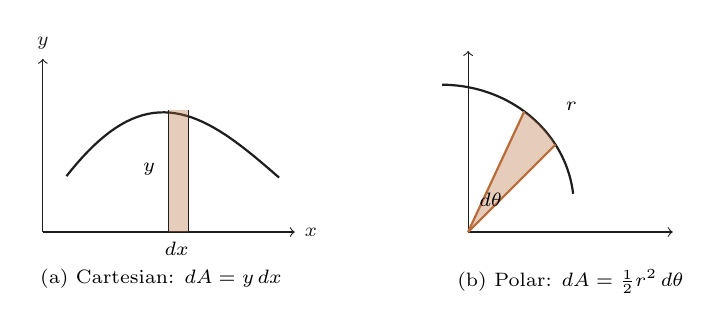
\begin{tikzpicture}[scale=1]
\begin{scope}
\draw[primary,->] (0,0) -- (3.2,0) node[right,font=\scriptsize] {$x$};
\draw[primary,->] (0,0) -- (0,2.2) node[above,font=\scriptsize] {$y$};
\draw[primary,thick,domain=0.3:3,samples=40] plot (\x, {0.3+1.6*sin(deg(\x/1.1))*exp(-\x/6)});
\fill[accent,opacity=0.35] (1.6,0) rectangle (1.85,1.55);
\draw[primary] (1.6,0) -- (1.6,1.55);
\draw[primary] (1.85,0) -- (1.85,1.55);
\node[below,font=\scriptsize] at (1.7,0) {$dx$};
\node[left,font=\scriptsize] at (1.55,0.8) {$y$};
\node[below,font=\scriptsize] at (1.5,-0.35) {(a) Cartesian: $dA = y\,dx$};
\end{scope}
\begin{scope}[xshift=5.4cm]
\coordinate (O) at (0,0);
\draw[primary,->] (O) -- (2.6,0) node[right,font=\scriptsize] {};
\draw[primary,->] (O) -- (0,2.3) node[above,font=\scriptsize] {};
\draw[primary,thick,domain=20:100,samples=40] plot ({\x}:{1.3+0.006*\x});
\fill[accent,opacity=0.35] (O) -- plot[domain=45:65,samples=15] ({\x}:{1.3+0.006*\x}) -- cycle;
\draw[accent,thick] (O) -- (45:1.57);
\draw[accent,thick] (O) -- (65:1.69);
\node[font=\scriptsize] at (55:0.5) {$d\theta$};
\node[right,font=\scriptsize] at (55:1.95) {$r$};
\node[below,font=\scriptsize] at (1.3,-0.35) {(b) Polar: $dA = \tfrac{1}{2}r^2\,d\theta$};
\end{scope}
\end{tikzpicture}
\end{center}


\section*{\color{primary} I. Core Formulas for Area (Cartesian \& Parametric)}

\textit{\small Context: Quadrature is the process of finding the area bounded by a contour. The fundamental approach is the limit of a sum of inscribed rectangles.}

\begin{center}
\begin{tabular}{@{}p{0.45\columnwidth} p{0.45\columnwidth}@{}}
\toprule
\textbf{Standard Cartesian} & \textbf{Parametric Form $(x(t), y(t))$} \\
\midrule
$A = \int_a^b y \, dx$ & $A = \int_{t_1}^{t_2} y(t) x'(t) \, dt$ \\
\midrule
\textbf{Between Two Curves} & \textbf{Arc Length Parameter $s$} \\
\midrule
$A = \int_a^b |y_1 - y_2| \, dx$ & $A = \int y \cos \gamma \, ds = \int x \sin \gamma \, ds$ \\
\bottomrule
\end{tabular}
\end{center}

\vspace{0.3cm}

\section*{\color{primary} II. Line Integrals \& Contour Forms}

\textit{\small Context: By applying Green's Theorem (or summing elementary sectors/triangles), the area of a closed contour can be evaluated as a line integral around its perimeter.}

\begin{center}
\begin{tabular}{@{}p{0.9\columnwidth}@{}}
\toprule
\textbf{\color{accent}Contour Integral Forms (Counter-Clockwise Traversal):} \\
$A = \oint -y \cos \gamma \, ds = \oint x \sin \gamma \, ds = \frac{1}{2} \oint (x \, dy - y \, dx)$ \\
\textit{\small where $\gamma$ is the angle the tangent makes with the positive x-axis.} \\
\bottomrule
\end{tabular}
\end{center}

\vspace{0.3cm}

\section*{\color{primary} III. Sectorial Areas (Polar Coordinates)}

\textit{\small Context: When the area is bounded by a curve $r=f(\theta)$ and two radii vectores, the elementary area is a circular sector $\frac{1}{2}r^2 d\theta$.}

\begin{center}
\begin{tabular}{@{}p{0.45\columnwidth} p{0.45\columnwidth}@{}}
\toprule
\textbf{Standard Polar} & \textbf{Cartesian Equivalent} \\
\midrule
$A = \frac{1}{2} \int_{\alpha}^{\beta} r^2 \, d\theta$ & $A = \frac{1}{2} \int_{\alpha}^{\beta} (x \, dy - y \, dx)$ \\
\midrule
\textbf{Substitution $v = y/x = \tan \theta$} & \textbf{Symmetry Rule} \\
\midrule
$A = \frac{1}{2} \int x^2 \, dv$ & If symmetric about initial line: $A = 2 \times \frac{1}{2} \int_0^{\alpha} r^2 \, d\theta$ \\
\bottomrule
\end{tabular}
\end{center}

\vspace{0.2cm}

\textit{\small Note on $v = \tan \theta$:} The substitution $v = y/x$ transforms the polar area integral into $\frac{1}{2} \int x^2 \, dv$. Care must be taken not to integrate through an infinite value of $v$ (which occurs when $\theta = \pi/2$ or odd multiples).


\section*{\color{primary} IV. High-Yield Memory Rules \& Precautions}

\textbf{1. Nodes and Self-Intersecting Curves}\\
If a closed curve crosses itself (has nodes/loops), a continuous line integral $\frac{1}{2} \oint (x \, dy - y \, dx)$ around the \textit{entire} perimeter yields the \textbf{algebraic difference} of the areas of the loops (odd loops minus even loops). 
\textit{Rule:} To find the total absolute area, you must isolate each loop, integrate separately, and sum their absolute values.

\textbf{2. Asymptotes and Infinite Ordinates}\\
If the curve has an asymptote or $y \to \infty$ at $x=c$, the area might still be finite. 
\textit{Rule:} If $y \sim \frac{A}{(x-c)^n}$ as $x \to c$, the principal value of the integral is finite if $n < 1$. Always separate the regions on opposite sides of the asymptote, evaluate their limits, and add the positive results.

\textbf{3. The "Pedal" and "Reciprocal" Spirals}\\
Frequently appear in Olympiad/bee contexts. 
\begin{itemize}[leftmargin=*, nosep]
    \item \textbf{\color{accent}Archimedean:} $r = a\theta \implies A = \frac{1}{3} a^2 \theta^3$
    \item \textbf{\color{accent}Reciprocal:} $r\theta = a \implies A = \frac{1}{2} a^2 \left(\frac{1}{\theta_1} - \frac{1}{\theta_2}\right)$
    \item \textbf{\color{accent}Logarithmic:} $r = a e^{\theta \cot \alpha} \implies A = \frac{1}{2} a^2 \cot \alpha (e^{2\theta \cot \alpha} - 1)$
\end{itemize}

\newpage

\begin{center}
    {\LARGE \bfseries \color{accent} Chapter XIII: Quadrature (II)}\\
    \vspace{0.2cm}
    {\color{accent}\rule{0.55\linewidth}{0.8pt}}
\end{center}
\vspace{0.35cm}

\begin{center}
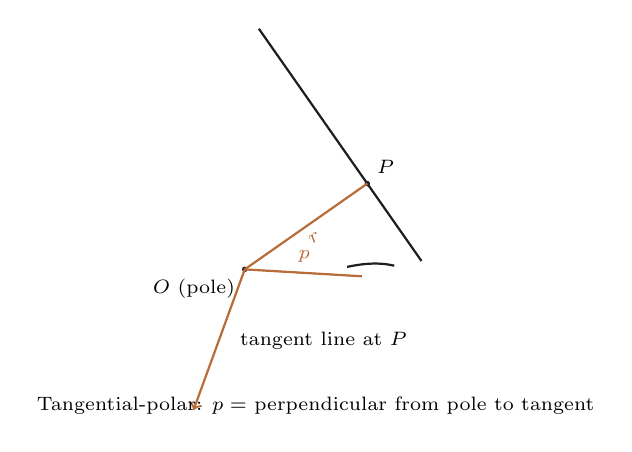
\begin{tikzpicture}[scale=1]
\draw[primary,thick,domain=0:340,samples=80] plot ({2+0.6*cos(2*\x)}:{1.6+0.3*sin(\x)});
\coordinate (O) at (0,0);
\fill[primary] (O) circle (1pt);
\node[below left,font=\scriptsize] at (O) {$O$ (pole)};
\coordinate (P) at (35:1.9);
\fill[primary] (P) circle (1pt);
\node[above right,font=\scriptsize] at (P) {$P$};
\draw[primary,thick] (P) -- ($(P)+(35+90:2.4)$) coordinate (Ta);
\draw[primary,thick] (P) -- ($(P)-(35+90:1.2)$) coordinate (Tb);
\draw[accent,thick] (O) -- (P) node[midway,below,font=\scriptsize,sloped] {$r$};
\draw[accent,thick,->] (O) -- ($(O)!1!90+35+90:(P)$);
\draw[primary,dashed] (O) -- ($(O)!(P)!90:(Ta)$) coordinate (F);
\draw[accent,thick] (O) -- (F) node[midway,above,sloped,font=\scriptsize] {$p$};
\node[font=\scriptsize] at (1.0,-0.9) {tangent line at $P$};
\node[below,font=\scriptsize] at (0.9,-1.5) {Tangential-polar: $p = $ perpendicular from pole to tangent};
\end{tikzpicture}
\end{center}


\section*{\color{primary} I. Core Area Formulas (Alternative Coordinates)}

\textit{\small Context: When a curve is defined by coordinates other than standard Cartesian or Polar, the area can still be evaluated by summing elementary triangles or sectors. Here, $p$ is the perpendicular from the pole to the tangent, $s$ is the arc length, $r$ is the radius vector, and $\psi$ is the tangent angle.}

\begin{center}
\begin{tabular}{@{}p{0.45\columnwidth} p{0.45\columnwidth}@{}}
\toprule
\textbf{Coordinate System} & \textbf{Area Formula} \\
\midrule
\textbf{Tangential-Polar $(p, s)$} & $A = \frac{1}{2} \int p \, ds$ \\
\textbf{Tangential-Polar $(p, \psi)$} & $A = \frac{1}{2} \int \left( p^2 + \left(\frac{dp}{d\psi}\right)^2 \right) d\psi$ \\
\textbf{Pedal Equation $(p, r)$} & $A = \frac{1}{2} \int \frac{p r}{\sqrt{r^2-p^2}} \, dr$ \\
\bottomrule
\end{tabular}
\end{center}

\vspace{0.2cm}

\textit{\small Caution: If the curve has points of inflection or nodes, $p$ or $\sqrt{r^2-p^2}$ may change sign. Integrate section by section and sum the absolute areas.}


\section*{\color{primary} II. Intrinsic Equations \& Swept Areas}

\subsection*{\color{secondary} Intrinsic Equation $s = f(\psi)$}
\textit{\small Context: The area bounded by the curve, an initial tangent, and a normal can be found via a double integral. For a closed oval, the limits are $0$ to $2\pi$.}
\begin{align*}
    A &= \int_0^\psi \int_0^{\psi'} f(\psi) f'(\psi) \cos \psi \sin \psi \, d\psi \, d\psi' \\
    \text{Or equivalently: } A &= \frac{1}{2} \int_0^{2\pi} \int_0^\psi f(x) \sin(\psi-x) \, dx \, d\psi
\end{align*}

\subsection*{\color{secondary} Area Swept by a "Tail"}
\textit{\small Context: If a line of variable length $\phi(s)$ is drawn along the tangent from the point of contact, the area swept out as the point moves along the curve is given by:}
\begin{align*}
    A_{\text{swept}} = \frac{1}{2} \int \{\phi(s)\}^2 \, d\psi
\end{align*}
\textit{\small If $\phi(s) = c$ (a constant tail), the swept area for a closed oval is exactly $\pi c^2$, the area of a circle of radius $c$.}

\section*{\color{primary} III. Pedal Curves \& Parallel Curves}

\subsection*{\color{secondary} Pedal of an Evolute}
\textit{\small Context: Beautiful geometric relations exist between a closed oval, its pedal curve, and the pedal of its evolute.}
\begin{itemize}[leftmargin=*, nosep]
    \item \textbf{Area of Pedal} = Area of Oval + Area between Oval and its Pedal.
    \item \textbf{Area of Pedal} = Area of Oval + Area of Pedal of Evolute.
    \item \textbf{\color{accent}Additional Identity:} Area of Pedal = $\frac{1}{2}$(Area of Oval) + $\frac{1}{2} \int \frac{ds}{p}$.
\end{itemize}

\subsection*{\color{secondary} Parallel Curves}
\textit{\small Context: A parallel curve is traced at a constant normal distance $c$ from the original curve. The area between a closed oval and its exterior/interior parallel curve is:}
\begin{align*}
    A_{\text{parallel}} = A_{\text{oval}} + cs \pm \pi c^2
\end{align*}
where $s$ is the perimeter of the oval.

\section*{\color{primary} IV. Locus of Pedal Origins (Steiner's Theorem)}

\textit{\small Context: If a point $P$ moves such that the area of the pedal curve of a closed oval with respect to $P$ remains constant, the locus of $P$ is a circle.}

\begin{center}
\begin{tabular}{@{}p{0.9\columnwidth}@{}}
\toprule
\textbf{The Minimum Pedal Area \& Centroid of Curvature} \\
\midrule
The center $\Omega$ of this circular locus is the origin that \textbf{minimizes} the pedal area. \\
Geometrically, $\Omega$ is the \textbf{centroid} of a material wire bent into the shape of the oval, \\
where the linear density at each point is proportional to its curvature $\kappa = 1/p$. \\
\textbf{\color{accent}Formula:} $A_P = A_{\min} + \pi \cdot d^2$, where $d$ is the distance from $P$ to $\Omega$. \\
\bottomrule
\end{tabular}
\end{center}

\vspace{0.3cm}

\newpage

\begin{center}
    {\LARGE \bfseries \color{accent} Chapter XIV: Quadrature (III)}\\
    \vspace{0.2cm}
    {\color{accent}\rule{0.55\linewidth}{0.8pt}}
\end{center}
\vspace{0.35cm}

\begin{center}
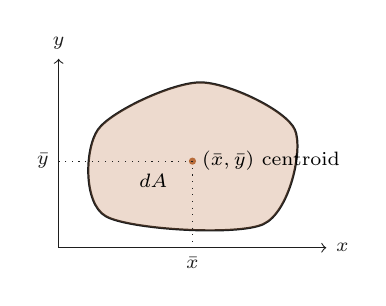
\begin{tikzpicture}
\draw[primary,->] (0,0) -- (3.4,0) node[right,font=\scriptsize]{$x$};
\draw[primary,->] (0,0) -- (0,2.4) node[above,font=\scriptsize]{$y$};
\draw[primary,thick] plot[smooth cycle] coordinates {(0.6,0.4) (2.6,0.3) (3.0,1.5) (1.8,2.1) (0.5,1.5)};
\fill[accent,opacity=0.25] plot[smooth cycle] coordinates {(0.6,0.4) (2.6,0.3) (3.0,1.5) (1.8,2.1) (0.5,1.5)};
\fill[accent] (1.7,1.1) circle (1.3pt);
\node[right,font=\scriptsize] at (1.7,1.1) {$(\bar{x},\bar{y})$ centroid};
\draw[primary,dotted] (1.7,1.1) -- (1.7,0) node[below,font=\scriptsize] {$\bar{x}$};
\draw[primary,dotted] (1.7,1.1) -- (0,1.1) node[left,font=\scriptsize] {$\bar{y}$};
\node[font=\scriptsize] at (1.2,0.85) {$dA$};
\end{tikzpicture}
\end{center}


\section*{\color{primary} I. Surface Integrals \& Centroids}

\textit{\small Context: When a plane area has a non-uniform surface density $\sigma(x,y)$, the mass and centroid cannot be found using simple 1D integrals. We must sum second-order infinitesimal elements $dm = \sigma \, dA$ over the 2D region using double integrals.}

\subsection*{\color{secondary} Cartesian Coordinates}
\begin{center}
\begin{tabular}{@{}p{0.45\columnwidth} p{0.45\columnwidth}@{}}
\toprule
\textbf{Mass} & \textbf{Centroid $(\bar{x}, \bar{y})$} \\
\midrule
$M = \iint \sigma(x,y) \, dx \, dy$ & $\bar{x} = \frac{1}{M} \iint x \sigma(x,y) \, dx \, dy$ \\
& $\bar{y} = \frac{1}{M} \iint y \sigma(x,y) \, dx \, dy$ \\
\bottomrule
\end{tabular}
\end{center}

\vspace{0.2cm}

\subsection*{\color{secondary} Polar Coordinates}
\textit{\small Context: The area element in polar coordinates is $dA = r \, dr \, d\theta$. The distance from the origin is simply $r$.}
\begin{center}
\begin{tabular}{@{}p{0.45\columnwidth} p{0.45\columnwidth}@{}}
\toprule
\textbf{Mass} & \textbf{Centroid $(\bar{x}, \bar{y})$} \\
\midrule
$M = \iint \sigma(r,\theta) \, r \, dr \, d\theta$ & $\bar{x} = \frac{1}{M} \iint r \cos\theta \, \sigma \, r \, dr \, d\theta$ \\
& $\bar{y} = \frac{1}{M} \iint r \sin\theta \, \sigma \, r \, dr \, d\theta$ \\
\bottomrule
\end{tabular}
\end{center}


\section*{\color{primary} II. Moments of Inertia}

\textit{\small Context: The moment of inertia about an axis is the sum of the mass elements multiplied by the square of their distance from that axis. For a lamina in the $xy$-plane, the distance to the $y$-axis is $x$, and to the $x$-axis is $y$.}

\begin{center}
\begin{tabular}{@{}p{0.45\columnwidth} p{0.45\columnwidth}@{}}
\toprule
\textbf{Cartesian} & \textbf{Polar} \\
\midrule
$I_y = \iint x^2 \sigma \, dx \, dy$ & $I_O = \iint r^2 \sigma \, r \, dr \, d\theta$ \\
$I_x = \iint y^2 \sigma \, dx \, dy$ & (About the origin / perpendicular to plane) \\
\midrule
\multicolumn{2}{c}{\textbf{\color{accent}Perpendicular Axis Theorem:} $I_O = I_x + I_y$} \\
\bottomrule
\end{tabular}
\end{center}

\vspace{0.3cm}

\section*{\color{primary} III. Trilinear \& Areal Coordinates}

\textit{\small Context: These coordinates are primarily used for the descriptive geometry of conics rather than direct metric evaluation. To find the area, it is almost always best to transform back to Cartesian coordinates, or use the specific Jacobian area elements shown below.}

\begin{center}
\begin{tabular}{@{}p{0.45\columnwidth} p{0.45\columnwidth}@{}}
\toprule
\textbf{Areal Coordinates $(x,y,z)$} & \textbf{Trilinear Coordinates $(\alpha,\beta,\gamma)$} \\
\midrule
$x + y + z = 1$ & $a\alpha + b\beta + c\gamma = 2\Delta$ \\
\midrule
\textbf{\color{accent}Area Element:} & \textbf{\color{accent}Area Element:} \\
$dA = 2\Delta \, dx \, dy$ & $dA = \sin C \, d\alpha \, d\beta$ \\
\bottomrule
\end{tabular}
\end{center}

\vspace{0.2cm}
\textit{\small Note: $\Delta$ is the area of the reference triangle, and $a,b,c$ are its side lengths.}

\section*{\color{primary} IV. Corresponding Points \& Areas}

\textit{\small Context: A powerful technique for evaluating the area of complex algebraic curves (like $(m^2x^2+n^2y^2)^2 = \dots$) is to map them to simpler curves (like circles) via an affine transformation.}

\begin{center}
\begin{tabular}{@{}p{0.9\columnwidth}@{}}
\toprule
\textbf{\color{accent}Theorem:} If the coordinates of a curve $f(x,y)=0$ are related to a second curve $f(\xi,\eta)=0$ by the transformation $x = m\xi$ and $y = n\eta$, then the area $A$ of the first curve is related to the area $A'$ of the second by: \\
$A = m \cdot n \cdot A'$ \\
\textit{\small This is a direct consequence of the Jacobian determinant of the transformation being constant ($mn$).} \\
\bottomrule
\end{tabular}
\end{center}

\vspace{0.3cm}

\newpage

\begin{center}
    {\LARGE \bfseries \color{accent} Chapter XV: Quadrature (IV)}\\
    \vspace{0.2cm}
    {\color{accent}\rule{0.55\linewidth}{0.8pt}}
\end{center}
\vspace{0.35cm}

\begin{center}
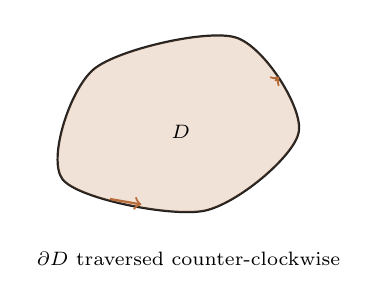
\begin{tikzpicture}
\draw[primary,thick] plot[smooth cycle] coordinates {(0.4,0.6) (2.2,0.2) (3.4,1.2) (2.6,2.4) (0.8,2.0)};
\fill[accent,opacity=0.2] plot[smooth cycle] coordinates {(0.4,0.6) (2.2,0.2) (3.4,1.2) (2.6,2.4) (0.8,2.0)};
\draw[accent,thick,->] (3.1,1.85) -- (3.15,1.9);
\draw[accent,thick,->] (1.0,0.35) -- (1.4,0.28);
\node[font=\scriptsize] at (1.9,1.2) {$D$};
\node[below,font=\scriptsize] at (2.0,-0.2) {$\partial D$ traversed counter-clockwise};
\end{tikzpicture}
\end{center}


\section*{\color{primary} I. Stokes' Theorem (Green's Theorem in the Plane)}

\textit{\small Context: Connects a line integral around a simple closed contour to a double integral over the plane region bounded by that contour. Highly useful for converting difficult line integrals into manageable area integrals, and vice versa.}

\begin{center}
\begin{tabular}{@{}p{0.9\columnwidth}@{}}
\toprule
\textbf{\color{accent}Theorem:} \\
$\displaystyle \oint_{\partial D} (u \, dx + v \, dy) = \iint_D \left( \frac{\partial v}{\partial x} - \frac{\partial u}{\partial y} \right) dx \, dy$ \\
\textit{\small where the line integral is taken counter-clockwise around the boundary $\partial D$.} \\
\bottomrule
\end{tabular}
\end{center}

\vspace{0.3cm}

\section*{\color{primary} II. Kinematic Area Theorems}

\subsection*{\color{secondary} Holditch's Theorem}
\textit{\small Context: If a chord of constant length slides with its endpoints on a closed convex curve, the area between the original curve and the curve traced by a point on the chord depends \textbf{only} on the lengths of the chord's segments, not on the shape of the original curve.}
\begin{align*}
    A_{\text{traced}} &= A_{\text{original}} - \pi a_1 a_2
\end{align*}
where $a_1, a_2$ are the lengths of the two segments of the chord.

\subsection*{\color{secondary} Leudesdorf's Theorem}
\textit{\small Context: Relates the area swept by a point $P$ rigidly attached to a moving triangle $ABC$ to the areas swept by the vertices.}
\begin{align*}
    [P] &= x[A] + y[B] + z[C] - \pi t^2
\end{align*}
where $x,y,z$ are the areal coordinates of $P$ w.r.t $ABC$, and $t^2$ is the power of $P$ with respect to the circumcircle of $ABC$ (if $P$ is outside; if inside, it's $-\pi \times \text{rectangle of segments}$).

\subsection*{\color{secondary} Kempe's Theorem}
\textit{\small Context: For a plane lamina moving in its own plane and returning to its original position, the locus of points on the lamina that trace curves of equal area is always a \textbf{circle}.}


\section*{\color{primary} III. Centroid of Moving Particles}

\subsection*{\color{secondary} Elliott's Theorem}
\textit{\small Context: The area $A_G$ described by the centroid of a system of $n$ moving particles is related to the individual areas and their relative motions. The particles do not need to be rigidly connected.}
\begin{align*}
    \left(\sum m_i\right) A_G &= \sum m_i A_i - \sum_{i<j} m_i m_j S_{ij}
\end{align*}
where $m_i$ are the masses, $A_i$ are the areas traced by each particle, and $S_{ij}$ is the relative area traced by $m_j$ with respect to $m_i$.

\section*{\color{primary} IV. Mechanical Integration (Amsler's Planimeter)}

\textit{\small Context: A mechanical device that measures the area of an arbitrary 2D shape by tracing its perimeter. It uses a rolling wheel to measure the normal displacement of a tracer arm.}

\begin{center}
\begin{tabular}{@{}p{0.45\columnwidth} p{0.45\columnwidth}@{}}
\toprule
\textbf{Pole Outside Contour} & \textbf{Pole Inside Contour} \\
\midrule
$A = l \cdot S$ & $A = l \cdot S + \pi r_0^2$ \\
\bottomrule
\end{tabular}
\end{center}

\vspace{0.2cm}
\textit{\small where $l$ is the length of the tracer arm, $S$ is the total distance registered by the rolling wheel, and $r_0$ is the radius of the "zero circle" (the circle traced when the wheel registers zero motion).}

\newpage

\begin{center}
    {\LARGE \bfseries \color{accent} Chapter XVI: Rectification (I)}\\
    \vspace{0.2cm}
    {\color{accent}\rule{0.55\linewidth}{0.8pt}}
\end{center}
\vspace{0.35cm}

\begin{center}
\begin{tikzpicture}
\draw[primary,->] (0,0) -- (3.6,0) node[right,font=\scriptsize]{$x$};
\draw[primary,->] (0,0) -- (0,2.4) node[above,font=\scriptsize]{$y$};
\draw[primary,thick,domain=0.3:3.2,samples=40] plot (\x,{0.3+0.28*\x*\x});
\coordinate (P) at (2.0,{0.3+0.28*4});
\coordinate (Q) at (2.35,{0.3+0.28*2.35*2.35});
\fill[primary] (P) circle (1pt);
\fill[primary] (Q) circle (1pt);
\draw[accent,thick] (P) -- (Q.center) node[midway,above,sloped,font=\scriptsize] {$ds$};
\draw[primary] (P) -- (Q.center |- P) coordinate(R);
\draw[primary] (R) -- (Q);
\node[below,font=\scriptsize] at ($(P)!0.5!(R)$) {$dx$};
\node[right,font=\scriptsize] at ($(R)!0.5!(Q)$) {$dy$};
\end{tikzpicture}
\end{center}


\section*{\color{primary} I. Core Arc Length Formulas}

\textit{\small Context: Rectification is the process of finding the arc length $s$ of a curve. The differential of arc length $ds$ is derived from the Pythagorean theorem applied to infinitesimal increments.}

\begin{center}
\begin{tabular}{@{}p{0.45\columnwidth} p{0.45\columnwidth}@{}}
\toprule
\textbf{Coordinate System} & \textbf{Differential $ds$ \& Integral $s$} \\
\midrule
\textbf{Cartesian $y=f(x)$} & $ds = \sqrt{1 + \left(\frac{dy}{dx}\right)^2} dx$ \\
\textbf{Cartesian $x=f(y)$} & $ds = \sqrt{1 + \left(\frac{dx}{dy}\right)^2} dy$ \\
\textbf{Parametric $x(t), y(t)$} & $ds = \sqrt{\left(\frac{dx}{dt}\right)^2 + \left(\frac{dy}{dt}\right)^2} dt$ \\
\textbf{Polar $r=f(\theta)$} & $ds = \sqrt{r^2 + \left(\frac{dr}{d\theta}\right)^2} d\theta$ \\
\textbf{Pedal $(p, r)$} & $ds = \frac{r}{\sqrt{r^2-p^2}} dr$ \\
\textbf{Tangential-Polar $(p, \chi)$} & $ds = \sqrt{1 + \left(\frac{dp}{d\chi}\right)^2} d\chi$ \\
\bottomrule
\end{tabular}
\end{center}

\vspace{0.3cm}

\section*{\color{primary} II. Centroids \& Moments of Inertia (Wires)}

\textit{\small Context: For a fine wire of line density $\rho$, the mass element is $dm = \rho \, ds$. These formulas are essential for physical applications of rectification.}

\begin{center}
\begin{tabular}{@{}p{0.45\columnwidth} p{0.45\columnwidth}@{}}
\toprule
\textbf{Centroid $(\bar{x}, \bar{y})$} & \textbf{Moments of Inertia} \\
\midrule
$\bar{x} = \frac{\int x \rho \, ds}{\int \rho \, ds}$ & $I_x = \int y^2 \rho \, ds$ \\
$\bar{y} = \frac{\int y \rho \, ds}{\int \rho \, ds}$ & $I_y = \int x^2 \rho \, ds$ \\
& $I_O = \int r^2 \rho \, ds$ \\
\bottomrule
\end{tabular}
\end{center}


\section*{\color{primary} III. Intrinsic Equations \& Evolutes}

\textit{\small Context: The intrinsic equation relates arc length $s$ and tangent angle $\psi$ (or curvature $\kappa = 1/\rho$). It defines the shape of a curve purely internally, without reference to any external coordinate axes.}

\subsection*{\color{secondary} Key Intrinsic Relations}
\begin{itemize}[leftmargin=*, nosep]
    \item \textbf{\color{accent}Radius of Curvature:} $\rho = \frac{ds}{d\psi}$
    \item \textbf{\color{accent}Pedal Distance:} $p = \int \cos \psi \, ds$ (from initial tangent)
    \item \textbf{\color{accent}Cartesian from Intrinsic:} $x = \int \cos \psi f'(\psi) d\psi$, \ $y = \int \sin \psi f'(\psi) d\psi$
\end{itemize}

\subsection*{\color{secondary} Arc of an Evolute}
\textit{\small Context: The evolute is the locus of centers of curvature. The length of an arc of the evolute is exactly equal to the difference of the radii of curvature of the original curve at the corresponding endpoints.}
\begin{align*}
    s_{\text{evolute}} &= \rho_1 - \rho_2
\end{align*}

\subsection*{\color{secondary} Whewell's Theorem}
\textit{\small Context: If you construct successive involutes of a given curve, keeping the "rectilinear tails" (the unwound string segments) equal, the ultimate limiting shape of these involutes is always an \textbf{equiangular spiral}.}

\section*{\color{primary} IV. Special Curves \& The Converse Problem}

\subsection*{\color{secondary} The Converse Problem}
Given $s$ as a function of $x, y, r,$ or $\theta$, the curve's equation can be found. E.g., if $s = f(x)$:
\begin{align*}
    y = \int \sqrt{\left(\frac{ds}{dx}\right)^2 - 1} \, dx
\end{align*}

\subsection*{\color{secondary} Cornu's Spiral (Clothoid)}
\textit{\small Context: Defined by the intrinsic equation $s^2 = a^2 \psi$. Its curvature is directly proportional to its arc length. It is fundamental in optics (Fresnel integrals) and modern railway/highway design to ensure smooth transition of centripetal acceleration.}

\newpage

\begin{center}
    {\LARGE \bfseries \color{accent} Chapter XVII: Rectification (II)}\\
    \vspace{0.2cm}
    {\color{accent}\rule{0.55\linewidth}{0.8pt}}
\end{center}
\vspace{0.35cm}

\begin{center}
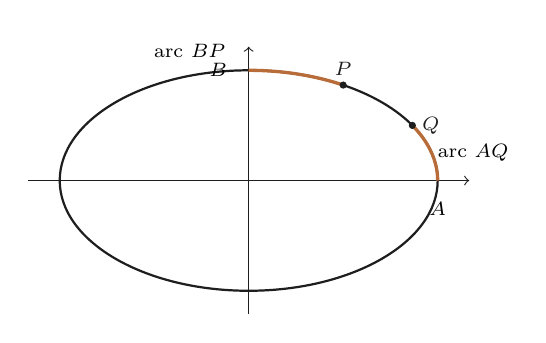
\begin{tikzpicture}
\draw[primary,thick] (0,0) ellipse (2.4 and 1.4);
\draw[primary,->] (-2.8,0) -- (2.8,0) node[right,font=\scriptsize]{};
\draw[primary,->] (0,-1.7) -- (0,1.7) node[above,font=\scriptsize]{};
\draw[accent,very thick,domain=60:90,samples=20] plot ({2.4*cos(\x)},{1.4*sin(\x)});
\draw[accent,very thick,domain=0:30,samples=20] plot ({2.4*cos(\x)},{1.4*sin(\x)});
\coordinate (P) at ({2.4*cos(60)},{1.4*sin(60)});
\coordinate (Q) at ({2.4*cos(30)},{1.4*sin(30)});
\fill[primary] (P) circle (1.3pt) node[above,font=\scriptsize]{$P$};
\fill[primary] (Q) circle (1.3pt) node[right,font=\scriptsize]{$Q$};
\node[below,font=\scriptsize] at (2.4,-0.15) {$A$};
\node[left,font=\scriptsize] at (-0.15,1.4) {$B$};
\node[font=\scriptsize] at (-0.75,1.65) {arc $BP$};
\node[font=\scriptsize] at (2.85,0.35) {arc $AQ$};
\end{tikzpicture}
\end{center}


\section*{\color{primary} I. The Ellipse \& Fagnano's Theorem}

\textit{\small Context: The rectification of the ellipse requires Legendre's Elliptic Integral of the Second Kind, $E(\phi, k)$. Unlike the circle, its perimeter cannot be expressed in elementary functions.}

\subsection*{\color{secondary} Arc Length Formulas}
\begin{center}
\begin{tabular}{@{}p{0.45\columnwidth} p{0.45\columnwidth}@{}}
\toprule
\textbf{From Minor Axis (Eccentric Angle $\theta$)} & \textbf{From Major Axis (Fagnano)} \\
\midrule
$s = a E(X, e)$ & $\text{Arc } BP - \text{Arc } AQ = \text{Tangent } QY$ \\
where $X = \frac{\pi}{2} - \theta$ & where $P, Q$ are related by confocal conics. \\
\midrule
\textbf{Perimeter Approximation} & \textbf{Fagnano Point Coordinates} \\
\midrule
$L \approx 2\pi a \left( 1 - \frac{1}{4}e^2 - \frac{3}{64}e^4 - \dots \right)$ & $x = \sqrt{\frac{a^3}{a+b}}, \quad y = \sqrt{\frac{b^3}{a+b}}$ \\
\bottomrule
\end{tabular}
\end{center}

\vspace{0.2cm}

\textbf{\color{accent}Fagnano's Theorem:} \textit{\small Shows that the difference of two arcs of an ellipse can be expressed algebraically. It essentially establishes the addition formula for elliptic integrals of the second kind. At the Fagnano point, $2 \text{arc } BF - \text{arc } AF = a - b$.}

\textbf{\color{accent}Graves's Theorem:} \textit{\small If tangents are drawn from any point on a confocal ellipse to the inner ellipse, the excess of the sum of these tangents over the intercepted arc is constant.}

\textbf{\color{accent}MacCullagh's Theorem:} \textit{\small The hyperbolic analogue to Graves's. If tangents are drawn from a point on a confocal hyperbola to the inner ellipse, the difference of the tangents equals the difference of the intercepted arcs.}


\section*{\color{primary} II. Hyperbola, Lemniscate \& Limaçon}

\subsection*{\color{secondary} Hyperbola ($x^2/a^2 - y^2/b^2 = 1$)}
\textit{\small Context: Arc measured from the vertex involves both $F$ (First Kind) and $E$ (Second Kind).}
\begin{align*}
    \text{Arc } AP &= PY + ae \left[ \cos^2\alpha F(\omega, \sin\alpha) - E(\omega, \sin\alpha) \right]
\end{align*}
where $\cot\alpha = b/a$, $\sin\omega = \frac{\sin\chi}{\sin\alpha}$, and $PY$ is the tangent length.

\subsection*{\color{secondary} Bernoulli's Lemniscate ($r^2 = a^2 \cos 2\theta$)}
\textit{\small Context: The perimeter is elegantly expressed using the Gamma function.}
\begin{align*}
    \text{Perimeter} &= 2a\sqrt{2} \int_0^{\pi/2} \frac{d\phi}{\sqrt{1 - \frac{1}{2}\sin^2\phi}} = a \frac{[\Gamma(1/4)]^2}{\sqrt{2\pi}} \approx 5.244116 a
\end{align*}

\subsection*{\color{secondary} Pascal's Limaçon ($r = a + b \cos\theta$)}
\textit{\small Context: The arc length is directly proportional to an elliptic integral of the second kind.}
\begin{align*}
    s &= 2(a+b) E\left(\frac{\theta}{2}, \frac{2\sqrt{ab}}{a+b}\right)
\end{align*}
\textit{\small Note: The arc of the Limaçon equals the arc of an ellipse with semi-major axis $2(a+b)$ and eccentricity $\frac{2\sqrt{ab}}{a+b}$.}

\section*{\color{primary} III. The Elastica \& Cotes's Spirals}

\subsection*{\color{secondary} The Elastica (Lintearia)}
\textit{\small Context: The curve assumed by a bent elastic rod or a flexible membrane holding water. Governed by $\rho y = c^2$.}
\begin{center}
\begin{tabular}{@{}p{0.45\columnwidth} p{0.45\columnwidth}@{}}
\toprule
\textbf{Undulating Case} & \textbf{Nodal Case} \\
\midrule
$s = c \, \text{sn}^{-1}\left(\sin\frac{\psi}{2}, \sin\frac{\alpha}{2}\right)$ & $s = c \, \text{cn}^{-1}\left(\cos\frac{\psi}{2}, \frac{1}{\sqrt{2}}\right)$ \\
$y = 2c \sin\frac{\alpha}{2} \text{cn}\left(u, \sin\frac{\alpha}{2}\right)$ & $y = 2a \, \text{dn}\left(u, \frac{1}{\sqrt{2}}\right)$ \\
\bottomrule
\end{tabular}
\end{center}

\subsection*{\color{secondary} Cotes's Spirals}
\textit{\small Context: Defined by the pedal equation $1/p^2 = A/r^2 + B$. Includes the equiangular and reciprocal spirals as degenerate cases.}
\begin{align*}
    \text{Reciprocal Spiral } (r\theta = a): \quad s &= a \left( \sqrt{1+\theta^2} + \log(\theta + \sqrt{1+\theta^2}) \right)
\end{align*}

\section*{\color{primary} IV. Bi-polar Coordinates \& Genocchi's Theorem}

\textit{\small Context: Using distances $r_1, r_2$ from two fixed poles $S, H$ (distance $2c$). Elliptic coordinates $\xi, \eta$ are defined by $r_1+r_2 = 2\xi$, $r_1-r_2 = 2\eta$.}

\begin{align*}
    c^2 ds^2 &= (\xi^2 - c^2) d\eta^2 + (c^2 - \eta^2) d\xi^2 \\
    \text{Area Element:} \quad 16\Delta^2 &= (2c+r_1+r_2)(-2c+r_1+r_2)(2c-r_1+r_2)(2c+r_1-r_2)
\end{align*}

\textbf{\color{accent}Genocchi's Theorem:} \textit{\small The arc of a Cartesian oval (defined by $l r_1 + m r_2 = n$) can be expressed in terms of exactly three elliptic arcs.}

\newpage

\begin{center}
    {\LARGE \bfseries \color{accent} Chapter XVIII: Rectification (III)}\\
    \vspace{0.2cm}
    {\color{accent}\rule{0.55\linewidth}{0.8pt}}
\end{center}
\vspace{0.35cm}

\begin{center}
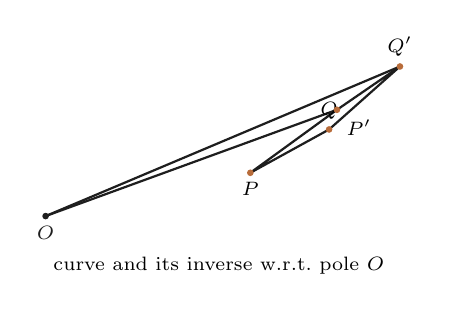
\begin{tikzpicture}
\coordinate (O) at (0,0);
\coordinate (P) at (2.6,0.55);
\coordinate (Q) at (3.6,1.1);
\coordinate (Pp) at (3.7,1.35);
\coordinate (Qp) at (4.5,1.9);
\draw[primary,thick] (O) -- (Qp);
\draw[primary,thick] (O) -- (Pp);
\draw[primary,thick] (P) -- (Q) -- (Qp) -- (Pp) -- cycle;
\fill[primary] (O) circle (1.2pt) node[below,font=\scriptsize]{$O$};
\fill[accent] (P) circle (1.2pt) node[below,font=\scriptsize,black]{$P$};
\fill[accent] (Q) circle (1.2pt) node[above,font=\scriptsize,black]{$Q$};
\fill[accent] (Pp) circle (1.2pt) node[below right,font=\scriptsize,black]{$P'$};
\fill[accent] (Qp) circle (1.2pt) node[above,font=\scriptsize,black]{$Q'$};
\node[below,font=\scriptsize] at (2.2,-0.4) {curve and its inverse w.r.t.\ pole $O$};
\end{tikzpicture}
\end{center}


\section*{\color{primary} I. Inverse Curves \& Bernoulli's Theorem}

\subsection*{\color{secondary} Arc of an Inverse Curve}
\textit{\small Context: Inversion with respect to a fixed point $O$ with constant $k$ maps a curve to its inverse. The arc length element transforms elegantly, allowing the rectification of the inverse to be found directly from the original curve.}
\begin{center}
\begin{tabular}{@{}p{0.45\columnwidth} p{0.45\columnwidth}@{}}
\toprule
\textbf{General Formula} & \textbf{Coordinate Modifications} \\
\midrule
$ds' = \frac{k^2}{r^2} ds$ & \textbf{\color{accent}Polar:} $s' = k^2 \int \frac{\sqrt{r^2 + (dr/d\theta)^2}}{r^2} d\theta$ \\
& \textbf{\color{accent}Pedal:} $s' = k^2 \int \frac{dr}{p\sqrt{r^2-p^2}}$ \\
& \textbf{\color{accent}Cartesian:} $s' = k^2 \int \frac{\sqrt{dx^2+dy^2}}{x^2+y^2}$ \\
\bottomrule
\end{tabular}
\end{center}

\vspace{0.3cm}

\subsection*{\color{secondary} John Bernoulli's Theorem}
\textit{\small Context: If a system of particles moves such that their tangents are always parallel, the centroid traces a new curve. By choosing the masses $m_i$ appropriately, this theorem generates an infinite number of new rectifiable curves from any given set of rectifiable curves.}
\begin{align*}
    ds_{\text{centroid}} &= \frac{\sum m_i ds_i}{\sum m_i}
\end{align*}
\textit{\small Note: If tangents are in opposite directions, the corresponding $ds_i$ must be taken with a negative sign.}


\section*{\color{primary} II. Symmetrical Ovoids \& Coordinate Systems}

\subsection*{\color{secondary} Ovoid with One Axis of Symmetry}
\textit{\small Context: For an ovoid with one axis of symmetry, consider the locus of the midpoints of chords whose endpoint tangents are parallel. This locus generally forms a tricuspidal curve.}
\begin{itemize}[leftmargin=*, nosep]
    \item \textbf{\color{accent}Cusps:} Occur where the opposite radii of curvature are equal.
    \item \textbf{\color{accent}Perimeter:} The perimeter of the tricuspidal locus equals half the difference of the sums of alternate arcs of the original ovoid, divided by the points where opposite tangents are parallel and radii of curvature are equal.
\end{itemize}

\subsection*{\color{secondary} Areal and Trilinear Coordinates}
\textit{\small Context: While not ideal for metrical purposes, arc length elements can be formulated for unicursal curves defined in these systems.}
\begin{align*}
    \textbf{\color{accent}Trilinear:} \quad ds^2 &= \frac{a^2}{16\Delta^2} (a \, d\alpha^2 + b \, d\beta^2 + c \, d\gamma^2 + 2\sqrt{bc}\cos A \, d\beta d\gamma + \dots) \\
    \textbf{\color{accent}Areal:} \quad ds^2 &= bc \cos A \, dx^2 + ca \cos B \, dy^2 + ab \cos C \, dz^2
\end{align*}

\section*{\color{primary} III. Generation of Rectifiable Curves}

\subsection*{\color{secondary} Connexion between Quadrature and Rectification}
\textit{\small Context: By constructing a new curve with the same abscissa $x$ but ordinate $\eta = a \sec \gamma$ (where $\gamma$ is the slope angle of the original curve), the area under the new curve equals $a \times$ (arc length of the original curve).}

\subsection*{\color{secondary} Parametric Class of Rectifiable Curves}
\textit{\small Context: By choosing arbitrary functions $F(t)$ and $f(t)$, we can generate curves whose arc lengths are trivially integrable.}
\begin{align*}
    x &= \int F(t) \cos f(t) \, dt, \quad y = \int F(t) \sin f(t) \, dt \implies ds = F(t) \, dt
\end{align*}

\subsection*{\color{secondary} Roberts' Theorem (Complex Transformation)}
\textit{\small Context: Using complex variables $u = x+iy$ and $v = x-iy$, if a curve satisfies $p(u)p(v) = 1$, a new curve with equal arc lengths can be derived by integrating powers of $p(u)$ and $p(v)$.}
\begin{align*}
    u' = \int [p(u)]^n \, du, \quad v' = \int [p(v)]^n \, dv \implies ds' = ds
\end{align*}

\subsection*{\color{secondary} Serret's Method}
\textit{\small Context: Serret demonstrated a process to generate purely algebraic curves that are rectifiable in terms of circular arcs (without elliptic functions) by integrating specific rational complex functions.}
\begin{align*}
    x+iy = C e^{i\omega} \int \frac{dz}{(z-a)^{m+1}(z+a)^{n+1}}
\end{align*}

\newpage

\begin{center}
    {\LARGE \bfseries \color{accent} Chapter XIX: Moving Curves}\\
    \vspace{0.2cm}
    {\color{accent}\rule{0.55\linewidth}{0.8pt}}
\end{center}
\vspace{0.35cm}

\begin{center}
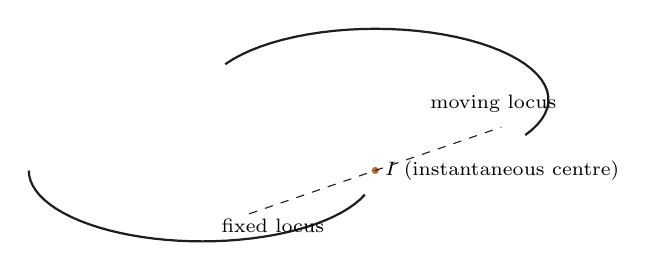
\begin{tikzpicture}
\draw[primary,thick,domain=180:340,samples=40] plot ({2.2*cos(\x)},{-1+0.9*sin(\x)});
\draw[primary,thick,domain=-30:150,samples=40] plot ({2.2+2.2*cos(\x)},{-1+0.9*sin(\x)+0.9});
\coordinate (I) at (2.2,-1);
\fill[accent] (I) circle (1.3pt) node[right,font=\scriptsize,black]{$I$ (instantaneous centre)};
\draw[primary,dashed] (0.6,-1.55) -- (3.8,-0.45);
\node[font=\scriptsize] at (0.9,-1.7) {fixed locus};
\node[font=\scriptsize] at (3.7,-0.15) {moving locus};
\end{tikzpicture}
\end{center}


\section*{\color{primary} I. Instantaneous Centre \& Kinematics}

\textit{\small Context: Any displacement of a plane lamina is equivalent to a rotation about an "Instantaneous Centre" (I). As the lamina moves, I traces a curve on the fixed plane and a corresponding curve on the moving lamina. The motion is kinematically equivalent to the rolling of the moving I-locus on the fixed I-locus without sliding.}

\subsection*{\color{secondary} Curvature of the I-Loci}
If $\rho_1$ and $\rho_2$ are the radii of curvature of the fixed and moving I-loci at the point of contact, and $\psi$ is the angle of the common tangent:
\begin{align*}
    \frac{d\psi}{ds} = \frac{1}{\rho_2} - \frac{1}{\rho_1}
\end{align*}
\textit{\small Note: Concavities in the same direction are assumed; signs must be adjusted if curves are convex/concave relative to the contact point.}


\section*{\color{primary} II. Roulettes and Glisettes}

\textit{\small Context: A \textbf{Roulette} is the path traced by a carried point. A \textbf{Glisette} is the envelope of a carried line. These are fundamental in kinematic geometry and gear design.}

\subsection*{\color{secondary} Curvature of an Envelope (Carried Curve)}
If a curve $\rho$ rolls on a fixed curve, the radius of curvature $R$ of the envelope of a carried curve $r$ is given by:
\begin{align*}
    \frac{\cos \phi}{R} - \frac{\cos \phi}{r} = \frac{1}{\rho} - \frac{1}{\rho_1} - \frac{1}{\rho_2}
\end{align*}
where $\phi$ is the angle the normal to the carried curve makes with the common normal.

\subsection*{\color{secondary} Steiner's \& Besant's Theorems (Rolling on a Straight Line)}
When a curve rolls on a fixed straight line:
\begin{itemize}[leftmargin=*, nosep]
    \item \textbf{\color{accent}Steiner's Theorem:} The arc of the roulette of a carried point is exactly equal to the corresponding arc of the \textbf{pedal} of the rolling curve with respect to that point.
    \item \textbf{\color{accent}Besant's Theorem:} The area swept out by the ordinate of the roulette is exactly \textbf{double} the corresponding sectorial area of the pedal curve.
\end{itemize}

\section*{\color{primary} III. Confocal Conics \& Rectifiable Arcs}

\textit{\small Context: Confocal conics share remarkable rectification properties discovered by Graves and MacCullagh, linking tangent lengths to arc lengths.}

\begin{center}
\begin{tabular}{@{}p{0.45\columnwidth} p{0.45\columnwidth}@{}}
\toprule
\textbf{Graves's Theorem (Ellipses)} & \textbf{MacCullagh's Theorem (Hyperbolas)} \\
\midrule
If tangents are drawn from any point on a confocal ellipse to an inner ellipse, the \textbf{excess} of the sum of the tangents over the intercepted arc is \textbf{constant}. & If tangents are drawn from a point on a confocal hyperbola to an inner ellipse, the \textbf{difference} of the tangents equals the \textbf{difference} of the intercepted arcs. \\
\bottomrule
\end{tabular}
\end{center}

\vspace{0.2cm}

\textit{\small Application: These theorems provide a physical "string construction" for drawing confocal conics and prove that the difference of arcs between Fagnano points on an ellipse is algebraically rectifiable.}

\section*{\color{primary} IV. Isoperimetric Companionship}

\textit{\small Context: Two curves are "isoperimetric companions" if they can be mapped such that corresponding arcs are exactly equal ($ds = ds'$), and the area under one relates to the sectorial area of the other. This allows the rectification of one curve to immediately yield the rectification of its companion.}

\begin{center}
\begin{tabular}{@{}p{0.45\columnwidth} p{0.45\columnwidth}@{}}
\toprule
\textbf{Fixed Curve} & \textbf{Isoperimetric Companion} \\
\midrule
Straight Line ($y = x \cot \alpha$) & Equiangular Spiral ($r = a e^{\theta \cot \alpha}$) \\
Straight Line ($r = c \sec \theta$) & Catenary ($y = c \cosh \frac{x}{c}$) \\
Parabola ($y^2 = 4ax$) & Archimedean Spiral ($r = 2a\theta$) \\
Cycloid & Cardioid \\
Ellipse & Rhodonea Curve \\
\bottomrule
\end{tabular}
\end{center}

\vspace{0.3cm}

\newpage

\begin{center}
    {\LARGE \bfseries \color{accent} Chapter XX: Rectification of Twisted Curves}\\
    \vspace{0.2cm}
    {\color{accent}\rule{0.55\linewidth}{0.8pt}}
\end{center}
\vspace{0.35cm}

\begin{center}
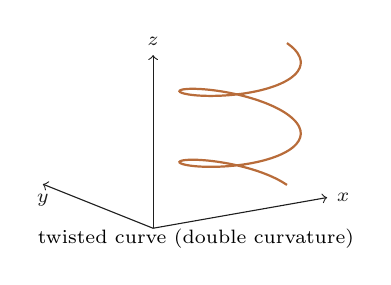
\begin{tikzpicture}[
  x={(0.85cm,0.15cm)}, y={(0,1cm)}, z={(-0.7cm,0.28cm)}
]
\draw[primary,->] (0,0,0) -- (2.6,0,0) node[right,font=\scriptsize]{$x$};
\draw[primary,->] (0,0,0) -- (0,2.2,0) node[above,font=\scriptsize]{$z$};
\draw[primary,->] (0,0,0) -- (0,0,2.0) node[below,font=\scriptsize]{$y$};
\draw[accent,thick,domain=0:720,samples=100,smooth] plot ({1.3+0.7*cos(\x)},{0.25+0.0025*\x},{0.7*sin(\x)});
\node[below,font=\scriptsize] at (1.3,-0.3,0.8) {twisted curve (double curvature)};
\end{tikzpicture}
\end{center}


\section*{\color{primary} I. Core Differential Formulas (3D Arc Length)}

\textit{\small Context: The rectification of a twisted curve (curve of double curvature) relies on the 3D Pythagorean theorem for infinitesimal displacements. The curve is typically defined either as the intersection of two surfaces or via parametric equations.}

\begin{center}
\begin{tabular}{@{}p{0.45\columnwidth} p{0.45\columnwidth}@{}}
\toprule
\textbf{Definition Type} & \textbf{Arc Length Element $ds$} \\
\midrule
\textbf{Cartesian Parametric} & $ds = \sqrt{\left(\frac{dx}{dt}\right)^2 + \left(\frac{dy}{dt}\right)^2 + \left(\frac{dz}{dt}\right)^2} dt$ \\
\textbf{Intersection of Surfaces} & $ds = \sqrt{dx^2 + dy^2 + dz^2}$ \\
$f(x,y,z)=0, F(x,y,z)=0$ & $\frac{dx}{J_1} = \frac{dy}{J_2} = \frac{dz}{J_3}$ \\
& where $J_i$ are the Jacobians of $(f, F)$ w.r.t $(y,z), (z,x), (x,y)$. \\
\bottomrule
\end{tabular}
\end{center}

\vspace{0.3cm}

\section*{\color{primary} II. Curvilinear Coordinates}

\begin{center}
\begin{tabular}{@{}p{0.45\columnwidth} p{0.45\columnwidth}@{}}
\toprule
\textbf{Cylindrical $(r, \theta, z)$} & \textbf{Spherical / Polar $(r, \theta, \phi)$} \\
\midrule
$ds = \sqrt{dr^2 + r^2 d\theta^2 + dz^2}$ & $ds = \sqrt{dr^2 + r^2 d\theta^2 + r^2 \sin^2\theta d\phi^2}$ \\
\midrule
\textbf{Pedal $(p, r)$ in 3D} & \textbf{Bi-polar $(r_1, r_2)$} \\
\midrule
$ds = \frac{r \, dr}{\sqrt{r^2-p^2}}$ & $c^2 ds^2 = (\xi^2-c^2)d\eta^2 + (c^2-\eta^2)d\xi^2$ \\
\textit{(Useful for curves on cones)} & \textit{(where $r_1+r_2=2\xi, r_1-r_2=2\eta$)} \\
\bottomrule
\end{tabular}
\end{center}

\vspace{0.3cm}

\section*{\color{primary} III. Geodesics \& The Helix}

\textit{\small Context: Geodesics are the shortest paths between points on a surface. A fundamental property is that if a surface is bent without stretching (inextensible deformation), its geodesics remain geodesics.}

\subsection*{\color{secondary} The Helix (Cylindrical Geodesic)}
\textit{\small Context: When a cylinder is unrolled into a flat plane, a helix becomes a straight line. Thus, the helix is the geodesic on a right circular cylinder.}
\begin{align*}
    x &= a \cos \theta, \quad y = a \sin \theta, \quad z = a \theta \tan \alpha \\
    ds &= a \sec \alpha \, d\theta \implies s = a \theta \sec \alpha
\end{align*}
where $\alpha$ is the constant angle the thread makes with the circular cross-section.


\section*{\color{primary} IV. Curves on Spheres \& Cones}

\subsection*{\color{secondary} Spherical Curves ($r=a$)}
\begin{align*}
    ds = a \sqrt{d\theta^2 + \sin^2\theta \, d\phi^2}
\end{align*}

\textbf{\color{accent}The Loxodrome (Rhumb Line):}\\
\textit{\small Context: A path on a sphere that cuts all meridians at a constant angle $\alpha$. Crucial in navigation (Mercator projection).}
\begin{align*}
    \phi &= \tan \alpha \log \tan\left(\frac{\theta}{2}\right) = \tan \alpha \cdot \text{gd}^{-1}(\theta)
\end{align*}

\subsection*{\color{secondary} Conical Curves ($\theta = \text{const} = \beta$)}
\textit{\small Context: A curve cutting all generators of a cone (semi-vertical angle $\beta$) at a constant angle $\alpha$. When the cone is unrolled, it becomes an equiangular spiral.}
\begin{align*}
    ds = \sqrt{dr^2 + r^2 \sin^2\beta \, d\phi^2}
\end{align*}

\section*{\color{primary} V. Inversion \& Projections}

\textit{\small Context: Inversion with respect to a fixed point (origin) with constant $k$ maps twisted curves to new twisted curves. Because inversion is a conformal mapping, it preserves the angles of intersection between curves.}

\begin{center}
\begin{tabular}{@{}p{0.9\columnwidth}@{}}
\toprule
\textbf{\color{accent}Inversion Arc Length Element:} \\
$ds' = \frac{k^2}{r^2} ds$ \\
\midrule
\textbf{\color{accent}Stereographic Projection:} \\
Maps spherical curves to planar curves. Preserves angles (orthogonal intersections remain orthogonal). \\
\bottomrule
\end{tabular}
\end{center}

\vspace{0.3cm}

\section*{\color{primary} VI. Bi-angular Coordinates}

\textit{\small Context: Uses angles $\theta_1, \theta_2$ that the radius vectors from two fixed poles make with the line joining the poles. Useful for curves defined by angular properties rather than distances.}
\begin{align*}
    c \, ds &= p_1 r_1 d\theta_2 - p_2 r_2 d\theta_1 \quad \text{or} \quad c \, ds = p_1 r_1 d\theta_2 + p_2 r_2 d\theta_1
\end{align*}
where $p_1, p_2$ are perpendiculars from the poles to the tangents.

\newpage

\begin{center}
    {\LARGE \bfseries \color{accent} Chapter XXI: Volumes \& Surfaces of Solids of Revolution}\\
    \vspace{0.2cm}
    {\color{accent}\rule{0.55\linewidth}{0.8pt}}
\end{center}
\vspace{0.35cm}

\begin{center}
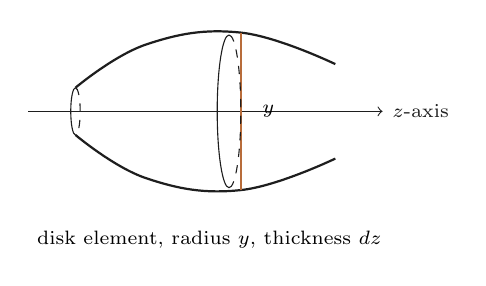
\begin{tikzpicture}
\draw[primary,->] (-0.3,0) -- (4.2,0) node[right,font=\scriptsize]{$z$-axis};
\draw[primary,thick] plot[smooth,tension=0.7] coordinates {(0.3,0.3) (1.2,0.85) (2.4,1.0) (3.6,0.6)};
\draw[primary,thick] plot[smooth,tension=0.7] coordinates {(0.3,-0.3) (1.2,-0.85) (2.4,-1.0) (3.6,-0.6)};
\draw[primary] (0.3,0.3) arc (90:270:0.06 and 0.3);
\draw[primary,dashed] (0.3,0.3) arc (90:-90:0.06 and 0.3);
\draw[accent,thick] (2.4,1.0) -- (2.4,-1.0);
\draw[primary] (2.25,0.97) arc (90:270:0.15 and 0.97);
\draw[primary,dashed] (2.25,0.97) arc (90:-90:0.15 and 0.97);
\node[right,font=\scriptsize] at (2.55,0) {$y$};
\node[below,font=\scriptsize] at (2.0,-1.4) {disk element, radius $y$, thickness $dz$};
\end{tikzpicture}
\end{center}


\section*{\color{primary} I. Volumes of Solids of Revolution}

\textit{\small Context: Formed by revolving a plane curve about an axis in its plane. The elementary volume is a disk of thickness $dz$ and radius $PN = y$.}

\begin{center}
\begin{tabular}{@{}p{0.45\columnwidth} p{0.45\columnwidth}@{}}
\toprule
\textbf{Axis of Revolution: $z$-axis} & \textbf{General Axis $AB$} \\
\midrule
$V = \pi \int_{z_1}^{z_2} y^2 \, dz$ & $V = \pi \int PN^2 \, d(ON)$ \\
\bottomrule
\end{tabular}
\end{center}

\vspace{0.3cm}

\section*{\color{primary} II. Surfaces of Revolution}

\textit{\small Context: The elementary surface area is a zone (frustum of a cone) traced by revolving the arc element $ds$ about the axis.}

\begin{center}
\begin{tabular}{@{}p{0.45\columnwidth} p{0.45\columnwidth}@{}}
\toprule
\textbf{Cartesian ($x$-axis)} & \textbf{Polar (Initial Line)} \\
\midrule
$S = 2\pi \int y \, ds = 2\pi \int y \sqrt{1 + \left(\frac{dy}{dx}\right)^2} dx$ & $S = 2\pi \int r \sin\theta \sqrt{r^2 + \left(\frac{dr}{d\theta}\right)^2} d\theta$ \\
\bottomrule
\end{tabular}
\end{center}

\vspace{0.3cm}

\section*{\color{primary} III. Centroids of Surfaces and Volumes}

\textit{\small Context: Assuming uniform density (or density symmetric about the axis). The centroid lies on the axis of revolution.}

\begin{center}
\begin{tabular}{@{}p{0.45\columnwidth} p{0.45\columnwidth}@{}}
\toprule
\textbf{Centroid of the Surface} & \textbf{Centroid of the Volume} \\
\midrule
$\bar{z} = \frac{\int z \cdot y \, ds}{\int y \, ds}$ & $\bar{z} = \frac{\int z \cdot y^2 \, dz}{\int y^2 \, dz}$ \\
\bottomrule
\end{tabular}
\end{center}

\vspace{0.3cm}


\section*{\color{primary} IV. Theorems of Pappus and Guldin}

\textit{\small Context: Relates the volume/surface of a solid of revolution to the centroid of the generating area/perimeter. Highly useful for avoiding direct integration when the centroid is known.}

\begin{center}
\begin{tabular}{@{}p{0.9\columnwidth}@{}}
\toprule
\textbf{\color{accent}Theorem I (Volume):} The volume of a solid generated by revolving a plane area about an external axis in its plane is equal to the area multiplied by the distance traveled by its centroid. \\
$V = A \cdot (2\pi \bar{y})$ \\
\midrule
\textbf{\color{accent}Theorem II (Surface):} The surface area generated by revolving a plane curve (perimeter) about an external axis is equal to the length of the curve multiplied by the distance traveled by its centroid. \\
$S = s \cdot (2\pi \bar{y})$ \\
\bottomrule
\end{tabular}
\end{center}

\vspace{0.2cm}

\textit{\small Note: If the axis cuts the area/curve, the theorems yield the \textbf{algebraic difference} of the volumes/surfaces generated by the portions on opposite sides.}

\subsection*{\color{secondary} Routh's Generalization}
\textit{\small Context: The axis of revolution need only be an \textbf{instantaneous axis}. If a plane lamina moves such that its plane is always perpendicular to the path of its centroid, the volume generated is Area $\times$ length of the path of the centroid.}

\subsection*{\color{secondary} Axis Not in the Plane}
\textit{\small Context: If the axis is parallel to the plane of the area but not in it, the volume is the same as if the revolution occurred about the \textbf{projection} of the axis onto the plane of the area. If the axis is inclined at an angle $\alpha$ to the plane, multiply the volume by $\cos\alpha$.}

\newpage

\begin{center}
    {\LARGE \bfseries \color{accent} Chapter XXII: Volumes, Surfaces \& Multiple Integration}\\
    \vspace{0.2cm}
    {\color{accent}\rule{0.55\linewidth}{0.8pt}}
\end{center}
\vspace{0.35cm}

\begin{center}
\begin{tikzpicture}[scale=1.1]
\coordinate (O) at (0,0);
\draw[primary,->] (O) -- (3,0) node[right,font=\scriptsize]{};
\draw[primary,->] (O) -- (0,2.6) node[above,font=\scriptsize]{};
\draw[primary,dashed] (O) -- (-1.6,-0.9);
\draw[primary,thick] (O) -- (2.35,0.85);
\draw[accent,thick] (O) -- (2.6,1.35);
\draw[primary,thick,domain=15:30,samples=10] plot ({1.3*cos(\x)},{1.3*sin(\x)});
\node[font=\scriptsize] at (1.55,0.45) {$d\theta$};
\node[right,font=\scriptsize] at (2.6,1.35) {volume element $r^2\sin\theta\,dr\,d\theta\,d\phi$};
\node[below,font=\scriptsize] at (1.2,-0.6) {spherical polar element};
\end{tikzpicture}
\end{center}


\section*{\color{primary} I. Volume by Triple Integration}

\textit{\small Context: The volume of a region is built by summing infinitesimal cuboids $\delta x\,\delta y\,\delta z$. The order of integration is chosen to match the geometry of the bounding surfaces.}

\begin{center}
\begin{tabular}{@{}p{0.45\columnwidth} p{0.45\columnwidth}@{}}
\toprule
\textbf{Cartesian} & \textbf{Cylindrical $(r,\theta,z)$} \\
\midrule
$V = \displaystyle\iiint dx\,dy\,dz$ & $V = \displaystyle\iiint r\,d\theta\,dr\,dz$ \\
\midrule
\multicolumn{2}{c}{\textbf{Spherical Polar $(r,\theta,\phi)$}} \\
\midrule
\multicolumn{2}{c}{$V = \displaystyle\iiint r^2 \sin\theta\,d\theta\,d\phi\,dr$} \\
\bottomrule
\end{tabular}
\end{center}

\vspace{0.2cm}

\textit{\small Note: When the volume between two surfaces $z=f_1(x,y)$ and $z=f_2(x,y)$ is needed, the innermost integral gives $V = \iint [f_1 - f_2]\,dx\,dy$.}

\vspace{0.3cm}

\section*{\color{primary} II. Mass, Centroid \& Moments of Inertia}

\textit{\small Context: Replace the volume element $dV$ by the mass element $\rho\,dV$ where $\rho(x,y,z)$ is the density. All mechanical quantities follow from summing $\rho\,dV$ weighted by the appropriate geometric factor.}

\begin{center}
\begin{tabular}{@{}p{0.45\columnwidth} p{0.45\columnwidth}@{}}
\toprule
\textbf{Mass \& Centroid} & \textbf{Moments of Inertia} \\
\midrule
$M = \iiint \rho\,dV$ & $A = \iiint \rho(y^2+z^2)\,dV$ \\
$\bar{x} = \frac{1}{M}\iiint \rho x\,dV$ & $B = \iiint \rho(z^2+x^2)\,dV$ \\
$\bar{y} = \frac{1}{M}\iiint \rho y\,dV$ & $C = \iiint \rho(x^2+y^2)\,dV$ \\
$\bar{z} = \frac{1}{M}\iiint \rho z\,dV$ & \\
\bottomrule
\end{tabular}
\end{center}

\vspace{0.2cm}

\textbf{\color{accent}Products of Inertia:} $D = \iiint \rho yz\,dV$, \ $E = \iiint \rho zx\,dV$, \ $F = \iiint \rho xy\,dV$.

\vspace{0.2cm}

\textbf{\color{accent}Routh's Mnemonic Rule:}\\
\textit{\small For a uniform body (disc, rectangle, sphere, ellipsoid), the moment of inertia about an axis of symmetry equals $M \times \frac{\text{sum of squares of perpendicular semi-axes}}{3, 4, \text{ or } 5}$ according as the body is rectangular, elliptical, or ellipsoidal.}


\section*{\color{primary} III. Surface Elements}

\textit{\small Context: The surface area element $dS$ is found by projecting onto a coordinate plane. If $\gamma$ is the angle between the normal and the $z$-axis, then $dx\,dy = dS \cos\gamma$.}

\begin{center}
\begin{tabular}{@{}p{0.45\columnwidth} p{0.45\columnwidth}@{}}
\toprule
\textbf{Cartesian $z=f(x,y)$} & \textbf{Cylindrical} \\
\midrule
$dS = \sqrt{1+p^2+q^2}\,dx\,dy$ & $dS = \sqrt{r^2 + \left(\frac{\partial z}{\partial \theta}\right)^2 + \left(\frac{\partial z}{\partial r}\right)^2 r^2}\,d\theta\,dr$ \\
$p = \frac{\partial z}{\partial x},\; q = \frac{\partial z}{\partial y}$ & \\
\midrule
\multicolumn{2}{c}{\textbf{Spherical Polar}} \\
\midrule
\multicolumn{2}{c}{$dS = \sqrt{r^4\sin^2\theta + r^2\sin^2\theta\left(\frac{\partial r}{\partial \theta}\right)^2 + r^2\left(\frac{\partial r}{\partial \phi}\right)^2}\,d\theta\,d\phi$} \\
\bottomrule
\end{tabular}
\end{center}

\vspace{0.3cm}

\section*{\color{primary} IV. Change of Variables}

\textit{\small Context: When switching to new coordinates $(u,v)$ or $(u,v,w)$, the area/volume element picks up the Jacobian determinant of the transformation.}

\begin{center}
\begin{tabular}{@{}p{0.45\columnwidth} p{0.45\columnwidth}@{}}
\toprule
\textbf{Area (2D)} & \textbf{Volume (3D)} \\
\midrule
$\displaystyle\iint f(x,y)\,dx\,dy = \iint F(u,v)\,J\,du\,dv$ & $\displaystyle\iiint f\,dx\,dy\,dz = \iiint F\,J\,du\,dv\,dw$ \\
$J = \frac{\partial(x,y)}{\partial(u,v)}$ & $J = \frac{\partial(x,y,z)}{\partial(u,v,w)}$ \\
\bottomrule
\end{tabular}
\end{center}

\vspace{0.2cm}

\textit{\small Note: If $J'$ is the Jacobian of $(u,v,w)$ w.r.t.\ $(x,y,z)$, then $JJ'=1$. Use whichever is easier to compute.}

\vspace{0.3cm}

\section*{\color{primary} V. Orthogonal Curvilinear Coordinates}

\textit{\small Context: For any three mutually orthogonal surfaces $f_1=\lambda$, $f_2=\mu$, $f_3=\nu$, the scale factors $h_1, h_2, h_3$ give $ds^2 = h_1^2 d\lambda^2 + h_2^2 d\mu^2 + h_3^2 d\nu^2$.}

\begin{align*}
    dV &= h_1 h_2 h_3\,d\lambda\,d\mu\,d\nu = \frac{\partial(x,y,z)}{\partial(\lambda,\mu,\nu)}\,d\lambda\,d\mu\,d\nu \\
    dS_\lambda &= h_2 h_3\,d\mu\,d\nu \quad \text{(element on surface $\lambda=\text{const}$)}
\end{align*}

\vspace{0.3cm}

\section*{\color{primary} VI. Solid Angles \& Gauss's Theorems}

\textit{\small Context: The solid angle $\omega$ subtended at $O$ by a surface element $dS$ is $d\omega = \frac{dS \cos\chi}{r^2}$, where $\chi$ is the angle between the inward normal and the radius vector.}

\begin{center}
\begin{tabular}{@{}p{0.9\columnwidth}@{}}
\toprule
\textbf{\color{accent}Gauss's Theorems:} \\
$\displaystyle\oint \cos\chi\,dS = \begin{cases} 4\pi & O \text{ inside the closed surface} \\ 2\pi & O \text{ on the surface (non-singular)} \\ 0 & O \text{ outside} \end{cases}$ \\
\bottomrule
\end{tabular}
\end{center}

\vspace{0.2cm}

\textbf{\color{accent}Volume via Surface Integral:}\\
\textit{\small The volume of a cone with vertex at $O$ and base $dS$ on the surface is $\frac{1}{3}p\,dS = \frac{1}{3}r\cos\chi\,dS$, giving:}
\begin{align*}
    V = \frac{1}{3}\oint p\,dS = \frac{1}{3}\oint r\cos\chi\,dS
\end{align*}

\vspace{0.3cm}

\section*{\color{primary} VII. Elliptic Coordinates}

\textit{\small Context: Three confocal quadrics $(\lambda, \mu, \nu)$ with $a>b>c$ provide orthogonal coordinates. Useful for ellipsoidal volumes and surfaces.}

\begin{align*}
    x^2 &= \frac{(a^2+\lambda)(a^2+\mu)(a^2+\nu)}{(a^2-b^2)(a^2-c^2)}, \quad \text{etc.} \\
    dV &= \frac{(\mu-\nu)(\nu-\lambda)(\lambda-\mu)}{8\sqrt{-\Delta_\lambda \Delta_\mu \Delta_\nu}}\,d\lambda\,d\mu\,d\nu
\end{align*}
where $\Delta_\lambda = (a^2+\lambda)(b^2+\lambda)(c^2+\lambda)$.

\textit{\small Limits for the ellipsoid $\frac{x^2}{a^2}+\frac{y^2}{b^2}+\frac{z^2}{c^2}=1$: $\lambda \in [0,-c^2]$, $\mu \in [-c^2,-b^2]$, $\nu \in [-b^2,-a^2]$.}
\end{document}

